\section{Datafit}
\label{sec:datafit}
The nominal model presented in \autoref{sec:nom_model} is now fit to the data in the reconstructed \pmu \cosmu variables, using the full 14 samples. Three Markov Chain Monte Carlo samples were run with different step-size tunings, acceptance rates and sample lengths, and a conservative 1/4 burn-in was used for all chains in \autoref{tab:mcmc_data}.
\begin{table}[h]
	\centering
	\begin{tabular}{l | c c c}
		\hline \hline
					& Steps		& Acceptance (\%) & Accepted steps \\
		\hline
		Tuned			& 800,000		& 24.0 	& 192,000 \\
		Long			& 3,000,000		& 6.2 	& 186,000 \\
		Short			& 1,600,000		& 6.2 	& 99,200 \\
		\hline \hline
	\end{tabular}
\caption{Different MCMC samples run for the data fit}
\label{tab:mcmc_data}
\end{table}

\autoref{tab:postfit_eventrate} shows the event rates per sample and total before and after the fit for the tuned MCMC, making correlated throws of the model to build the errors using the prior predictive method and the posterior predictive method, outlined earlier. 

We see very good agreement with the overall event rate (64768 data vs 64761.40 post-fit) and the CC0$\pi$ samples. The total sample contribution to the test-statistic\footnote{Excluding the penalty term from the priors} moves from 2539.08 to 1733.08. For the samples, we generally see good effect on targets, with FGD2 CC0$\pi$ decreasing the statistic by factor 2. Interestingly, FGD1 CCOther sees a noticeably smaller improvement than FGD2 (273.39 to 224.02 vs 277.96 to 171.17), indicating some tension in the fit. The uncertainty on the predictions decrease remarkably post-fit too: for the 0$\pi$ selections we go from an uncertainty of 2094.2 to 120.0, and overall from 6666.8 to 255.2. 

Compared to the expected Asimov prior predictive in \autoref{tab:asimov_prior_pred} and the posterior predictive in \autoref{tab:asimov_posterior_pred} the data fit uncertainties on the total event rates largely agree with the expectation. For both the prior and posterior predictive, the uncertainties from the data fit are within 10\% of the Asimov fit.
\begin{sidewaystable}
	\centering
		\begin{tabular}{ l | c c c | c c }
			\hline
			\hline
			Sample 			& \multicolumn{3}{c|}{Event rate} & \multicolumn{2}{c}{$-2\ln\mathcal{L}_S$} \\
							& Data	& Prior & Posterior & Prior & Posterior \\
                        \hline
			FGD1 0$\pi$ 	& 17136	& $16837.5\pm2094.2$ 	& $17122.9\pm120.0$ & 272.22  & 172.21 	\\ 
			FGD1 1$\pi$ 	& 3954 	& $4438.8\pm482.9$	& $4053.8\pm54.3$  & 259.65  & 164.04 	\\ 
			FGD1 Other 		& 4149 	& $3974.0\pm516.8$	& $4103.7\pm58.8$  & 273.39  & 224.03 	\\ 
                        \hline
			FGD2 0$\pi$ 	& 17443 & $16952.1\pm2072.6$	& $17501.5\pm122.5$ & 303.62  & 166.15 	\\ 
			FGD2 1$\pi$ 	& 3366 	& $3613.8\pm400.3$	& $3409.4\pm48.2$  & 228.72 & 162.71 	\\ 
			FGD2 Other 		& 4075 	& $3602.5\pm463.1$	& $3917.8\pm50.8$  & 277.96  & 171.17 	\\ 
                        \hline
			FGD1 1Trk 	& 3527 	& $3688.8\pm477.3$	& $3509.6\pm50.1$  & 156.19  & 117.80 	\\ 
			FGD1 NTrk 	& 1054 	& $1091.3\pm134.9$	& $1062.7\pm21.9$  & 109.59  & 76.50 	\\ 
			FGD2 1Trk 	& 3732 	& $3714.0\pm471.6$	& $3678.7\pm51.3$  & 169.17  & 129.84 	\\ 
			FGD2 NTrk 	& 1026 	& $1102.2\pm129.6$	& $1108.4\pm23.5$  & 89.74   & 80.34 	\\ 
                        \hline
			FGD1 \numu 1Trk 	& 1363 	& $1309.4\pm142.4$	& $1348.3\pm23.1$  & 88.42   & 66.51 	\\ 
			FGD1 \numu NTrk 	& 1370 	& $1376.8\pm153.9$	& $1359.1\pm26.9$  & 99.54   & 61.75 	\\ 
            FGD2 \numu 1Trk 	& 1320 	& $1303.4\pm139.7$	& $1323.1\pm23.8$  & 92.56   & 64.34 	\\ 
			FGD2 \numu NTrk		& 1253 	& $1263.1\pm139.7$	& $1265.9\pm24.2$  & 118.31  & 75.70 	\\ 
                        \hline
			Total 		& 64768 & $64603.2\pm6666.8$	& $64761.1\pm255.2$ & 2539.08 & 1733.08 \\
                        \hline
                        \hline
		\end{tabular}
	\caption{Event rate and test-statistic for data, pre-fit MC and post-fit MC broken by sample}
	\label{tab:postfit_eventrate}
\end{sidewaystable}

\autoref{fig:flux_data_fhc} shows the FHC flux parameters after the fit to data for the different chains. As expected and seen in the Asimov studies, the SK parameters closely follow the ND280 parameters. The parameters mostly sit within 1$\sigma$ of the prior, with the largest deviation around $E_\nu \sim 0.6-1.0\text{ GeV}$, where the flux normalisation drops sharply to 0.88 and returns to around nominal at $E_\nu\sim1.5\text{ GeV}$. At higher energies the flux normalisation decreases again to around 0.94. The parameters barely go above the priorexcept for \nue at 2 GeV and the high energy \nuebar parameters, although they still sit within one sigma of the central value of the prior.
\begin{figure}[h]
	\begin{subfigure}[t]{0.10\textwidth}
		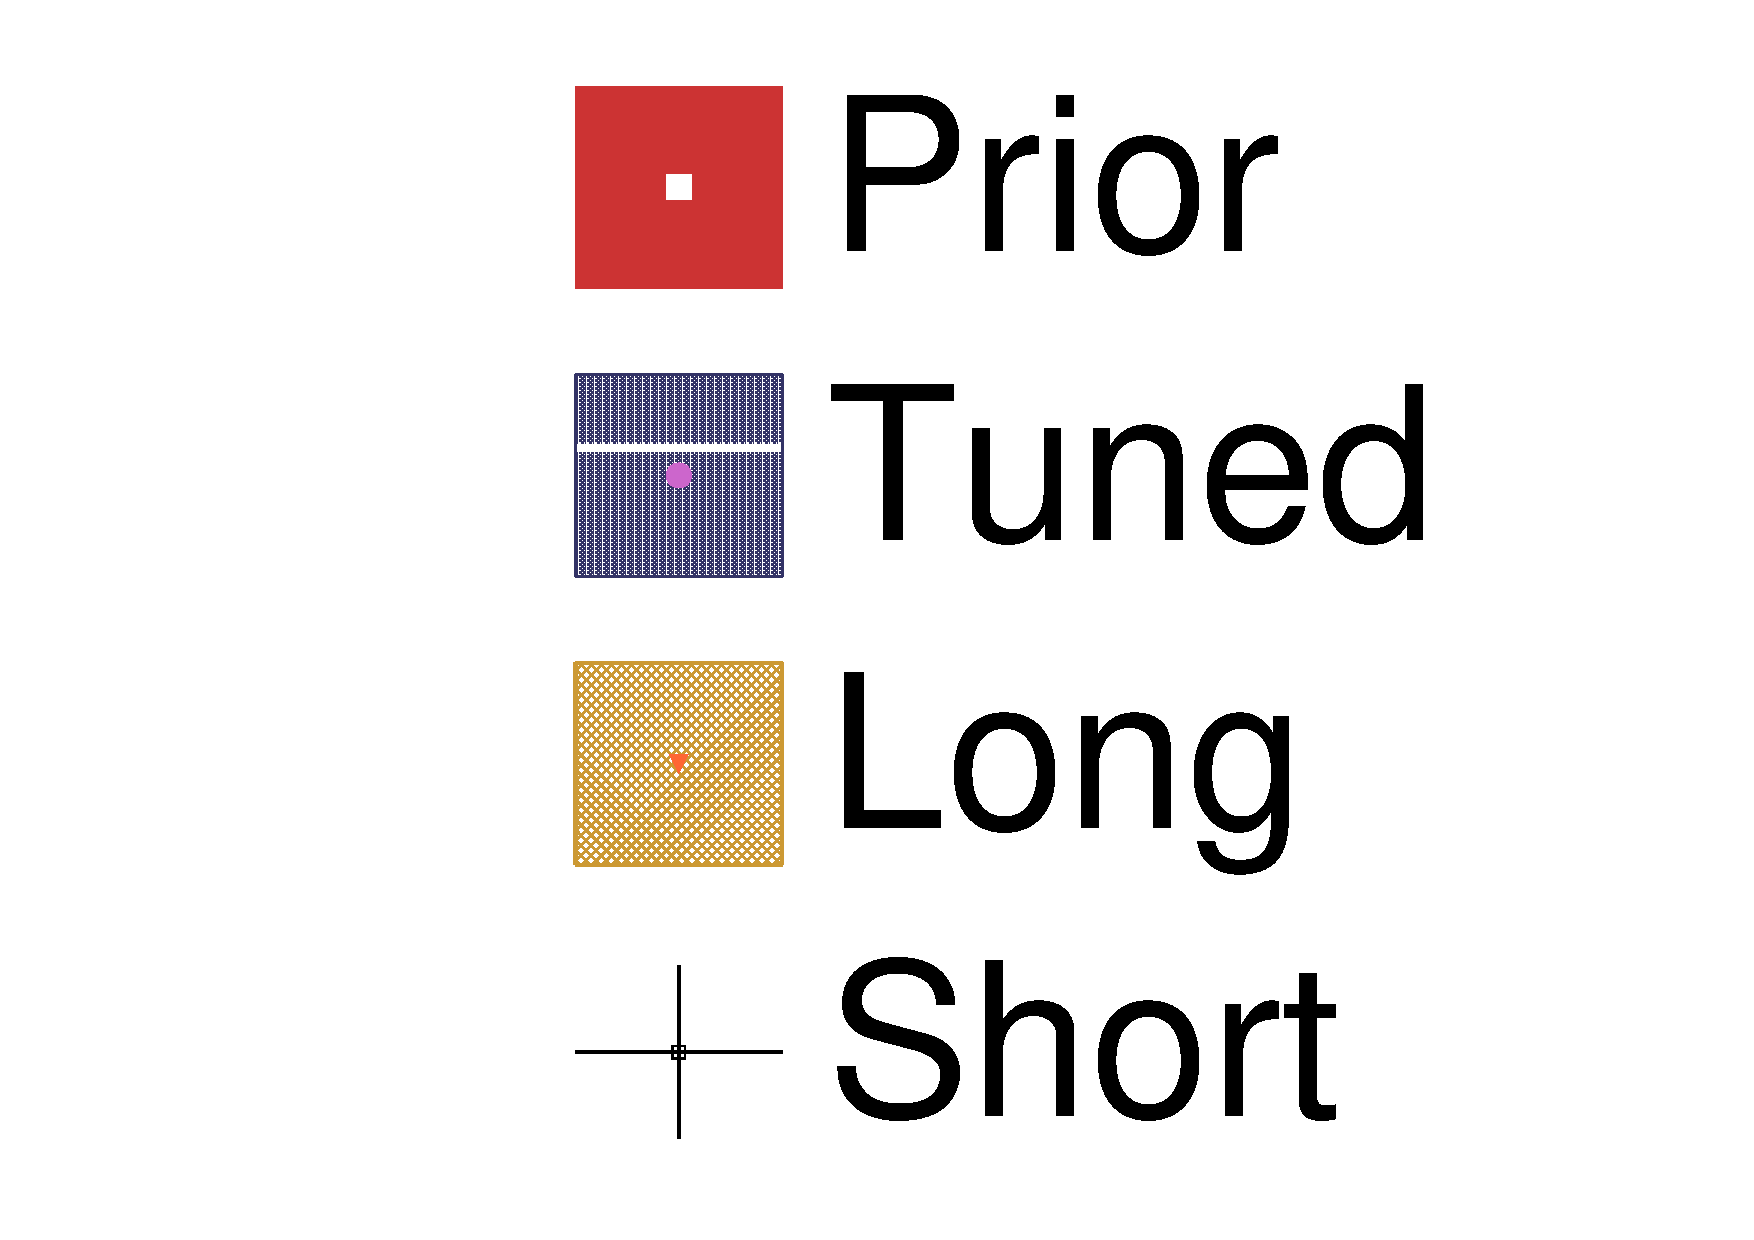
\includegraphics[width=\textwidth, trim={0mm 0mm 0mm 0mm}, clip,page=1]{figures/mach3/data/2017b_NewData_NewDet_UpdXsecStep_2Xsec_4Det_5Flux_0_2017b_June_NewDet_merge_2017b_NewDet_June_Long_0}
	\end{subfigure}
	
	\begin{subfigure}[t]{0.24\textwidth}
		\includegraphics[width=\textwidth, trim={0mm 0mm 0mm 0mm}, clip,page=2]{figures/mach3/data/2017b_NewData_NewDet_UpdXsecStep_2Xsec_4Det_5Flux_0_2017b_June_NewDet_merge_2017b_NewDet_June_Long_0}
	\end{subfigure}
	\begin{subfigure}[t]{0.24\textwidth}
		\includegraphics[width=\textwidth, trim={0mm 0mm 0mm 0mm}, clip,page=3]{figures/mach3/data/2017b_NewData_NewDet_UpdXsecStep_2Xsec_4Det_5Flux_0_2017b_June_NewDet_merge_2017b_NewDet_June_Long_0}
	\end{subfigure}
	\begin{subfigure}[t]{0.24\textwidth}
		\includegraphics[width=\textwidth, trim={0mm 0mm 0mm 0mm}, clip,page=4]{figures/mach3/data/2017b_NewData_NewDet_UpdXsecStep_2Xsec_4Det_5Flux_0_2017b_June_NewDet_merge_2017b_NewDet_June_Long_0}
	\end{subfigure}
	\begin{subfigure}[t]{0.24\textwidth}
		\includegraphics[width=\textwidth, trim={0mm 0mm 0mm 0mm}, clip,page=5]{figures/mach3/data/2017b_NewData_NewDet_UpdXsecStep_2Xsec_4Det_5Flux_0_2017b_June_NewDet_merge_2017b_NewDet_June_Long_0}
	\end{subfigure}
	
	\begin{subfigure}[t]{0.24\textwidth}
		\includegraphics[width=\textwidth, trim={0mm 0mm 0mm 0mm}, clip,page=10]{figures/mach3/data/2017b_NewData_NewDet_UpdXsecStep_2Xsec_4Det_5Flux_0_2017b_June_NewDet_merge_2017b_NewDet_June_Long_0}
	\end{subfigure}
	\begin{subfigure}[t]{0.24\textwidth}
		\includegraphics[width=\textwidth, trim={0mm 0mm 0mm 0mm}, clip,page=11]{figures/mach3/data/2017b_NewData_NewDet_UpdXsecStep_2Xsec_4Det_5Flux_0_2017b_June_NewDet_merge_2017b_NewDet_June_Long_0}
	\end{subfigure}
	\begin{subfigure}[t]{0.24\textwidth}
		\includegraphics[width=\textwidth, trim={0mm 0mm 0mm 0mm}, clip,page=12]{figures/mach3/data/2017b_NewData_NewDet_UpdXsecStep_2Xsec_4Det_5Flux_0_2017b_June_NewDet_merge_2017b_NewDet_June_Long_0}
	\end{subfigure}
	\begin{subfigure}[t]{0.24\textwidth}
		\includegraphics[width=\textwidth, trim={0mm 0mm 0mm 0mm}, clip,page=13]{figures/mach3/data/2017b_NewData_NewDet_UpdXsecStep_2Xsec_4Det_5Flux_0_2017b_June_NewDet_merge_2017b_NewDet_June_Long_0}
	\end{subfigure}
	\caption{FHC flux parameters after the data fit for different MCMC chains}
	\label{fig:flux_data_fhc}
\end{figure}

\autoref{fig:flux_data_rhc} shows the RHC flux parameters post-fit. For \numubar we see a decrease in the normalisation at low energies to approximately 0.96, which increases to the nominal at 0.6 GeV. At higher energies the normalisations go back to around 0.96. The only increase observed are the \nuebar parameters around 0.6 GeV. No parameters leave the 1$\sigma$ prior.
\begin{figure}[h]
	\begin{subfigure}[t]{0.24\textwidth}
		\includegraphics[width=\textwidth, trim={0mm 0mm 0mm 0mm}, clip,page=6]{figures/mach3/data/2017b_NewData_NewDet_UpdXsecStep_2Xsec_4Det_5Flux_0_2017b_June_NewDet_merge_2017b_NewDet_June_Long_0}
	\end{subfigure}
	\begin{subfigure}[t]{0.24\textwidth}
		\includegraphics[width=\textwidth, trim={0mm 0mm 0mm 0mm}, clip,page=7]{figures/mach3/data/2017b_NewData_NewDet_UpdXsecStep_2Xsec_4Det_5Flux_0_2017b_June_NewDet_merge_2017b_NewDet_June_Long_0}
	\end{subfigure}
	\begin{subfigure}[t]{0.24\textwidth}
		\includegraphics[width=\textwidth, trim={0mm 0mm 0mm 0mm}, clip,page=8]{figures/mach3/data/2017b_NewData_NewDet_UpdXsecStep_2Xsec_4Det_5Flux_0_2017b_June_NewDet_merge_2017b_NewDet_June_Long_0}
	\end{subfigure}
	\begin{subfigure}[t]{0.24\textwidth}
		\includegraphics[width=\textwidth, trim={0mm 0mm 0mm 0mm}, clip,page=9]{figures/mach3/data/2017b_NewData_NewDet_UpdXsecStep_2Xsec_4Det_5Flux_0_2017b_June_NewDet_merge_2017b_NewDet_June_Long_0}
	\end{subfigure}
	
	\begin{subfigure}[t]{0.24\textwidth}
		\includegraphics[width=\textwidth, trim={0mm 0mm 0mm 0mm}, clip,page=14]{figures/mach3/data/2017b_NewData_NewDet_UpdXsecStep_2Xsec_4Det_5Flux_0_2017b_June_NewDet_merge_2017b_NewDet_June_Long_0}
	\end{subfigure}
	\begin{subfigure}[t]{0.24\textwidth}
		\includegraphics[width=\textwidth, trim={0mm 0mm 0mm 0mm}, clip,page=15]{figures/mach3/data/2017b_NewData_NewDet_UpdXsecStep_2Xsec_4Det_5Flux_0_2017b_June_NewDet_merge_2017b_NewDet_June_Long_0}
	\end{subfigure}
	\begin{subfigure}[t]{0.24\textwidth}
		\includegraphics[width=\textwidth, trim={0mm 0mm 0mm 0mm}, clip,page=16]{figures/mach3/data/2017b_NewData_NewDet_UpdXsecStep_2Xsec_4Det_5Flux_0_2017b_June_NewDet_merge_2017b_NewDet_June_Long_0}
	\end{subfigure}
	\begin{subfigure}[t]{0.24\textwidth}
		\includegraphics[width=\textwidth, trim={0mm 0mm 0mm 0mm}, clip,page=17]{figures/mach3/data/2017b_NewData_NewDet_UpdXsecStep_2Xsec_4Det_5Flux_0_2017b_June_NewDet_merge_2017b_NewDet_June_Long_0}
	\end{subfigure}
	\caption{RHC flux parameters after the data fit for different MCMC chains}
	\label{fig:flux_data_rhc}
\end{figure}

\autoref{fig:xsec_data} show the interaction parameters after the fit, where we expect most of the parameter movement to happen. The largest deviations from the priors are seen for $M_A^{QE}$ and BeRPA B, followed by $M_A^{RES}$. 

The shift in $M_A^{QE}$ is expected since the ``prior'' value is from tunes to nuclear data, which historically inflates the value when not using adequate reasonable nuclear effects, such as 2p2h\red{cite niwg paper}. The parameterisation in these fits include such models, so uses a flat prior on $M_A^{QE}$ which in this fit is driven downwards toward values obtained from fits to nucleon data\red{cite some MAQE fit paper, Patrick's thesis?}. The post-fit value in real units is $M_A^{QE}=1.12\pm0.07\text{ GeV}$.

The BeRPA B shifts---and the remaining BeRPA shifts: BeRPA A at upper edge, BeRPA D at lower edge of the prior uncertainty---is more worrisome. The low $Q^2$ parameters BeRPA A and BeRPA B are being pushed above their pre-fit $1\sigma$ uncertainties, indicating that the ND280 data has more events than the Monte-Carlo at low $Q^2$, possibly forcing a shape that isn't ``RPA-like''. \autoref{fig:berpa_data} shows the BeRPA weight being applied for every step in the data and Asimov chains: the nominal shape (present in the Asimov) is heavily distorted in the data fit, in which a large weight at low $Q^2$ is strongly favoured and there is less constraint above $Q^2=0.5\text{ GeV}^2$.

The $M_A^{RES}$ parameter is pushed far from the bubble chamber tuned values (from $M_A^{RES}=1.07\pm0.15$ to $0.806\pm0.04$), whereas the other single pion production parameters are mostly in check. The may indicate sweeping up unmodelled nuclear effects (often approximately a function of $Q^2$) into the $M_A^{RES}$ parameter.

We note an interesting 2p2h normalisation, in which $\nu$ events pulls the normalisation to 1.6, whereas $\bar{\nu}$ normalisation is 0.8, indicating some $\nu$ vs $\bar{\nu}$ tension in 2p2h. The 2p2h shape parameters are pushed against their upper boundary, preferring a ``delta-like'' $q_0-q_3$ phase space, again indicating the 2p2h model does not entirely agree with ND280 data.

\begin{figure}[h]
	\begin{subfigure}[t]{0.49\textwidth}
		\includegraphics[width=\textwidth, trim={0mm 0mm 0mm 0mm}, clip,page=18]{figures/mach3/data/2017b_NewData_NewDet_UpdXsecStep_2Xsec_4Det_5Flux_0_2017b_June_NewDet_merge_2017b_NewDet_June_Long_0}
	\end{subfigure}
	\begin{subfigure}[t]{0.49\textwidth}
		\includegraphics[width=\textwidth, trim={0mm 0mm 0mm 0mm}, clip,page=19]{figures/mach3/data/2017b_NewData_NewDet_UpdXsecStep_2Xsec_4Det_5Flux_0_2017b_June_NewDet_merge_2017b_NewDet_June_Long_0}
	\end{subfigure}
	
	\begin{subfigure}[t]{0.49\textwidth}
		\includegraphics[width=\textwidth, trim={0mm 0mm 0mm 0mm}, clip,page=20]{figures/mach3/data/2017b_NewData_NewDet_UpdXsecStep_2Xsec_4Det_5Flux_0_2017b_June_NewDet_merge_2017b_NewDet_June_Long_0}
	\end{subfigure}
	\begin{subfigure}[t]{0.49\textwidth}
		\includegraphics[width=\textwidth, trim={0mm 0mm 0mm 0mm}, clip,page=21]{figures/mach3/data/2017b_NewData_NewDet_UpdXsecStep_2Xsec_4Det_5Flux_0_2017b_June_NewDet_merge_2017b_NewDet_June_Long_0}
	\end{subfigure}
	\caption{Interaction parameters after the data fit for different MCMC chains}
	\label{fig:xsec_data}
\end{figure}

\begin{figure}[h]
	\begin{subfigure}[t]{0.49\textwidth}
		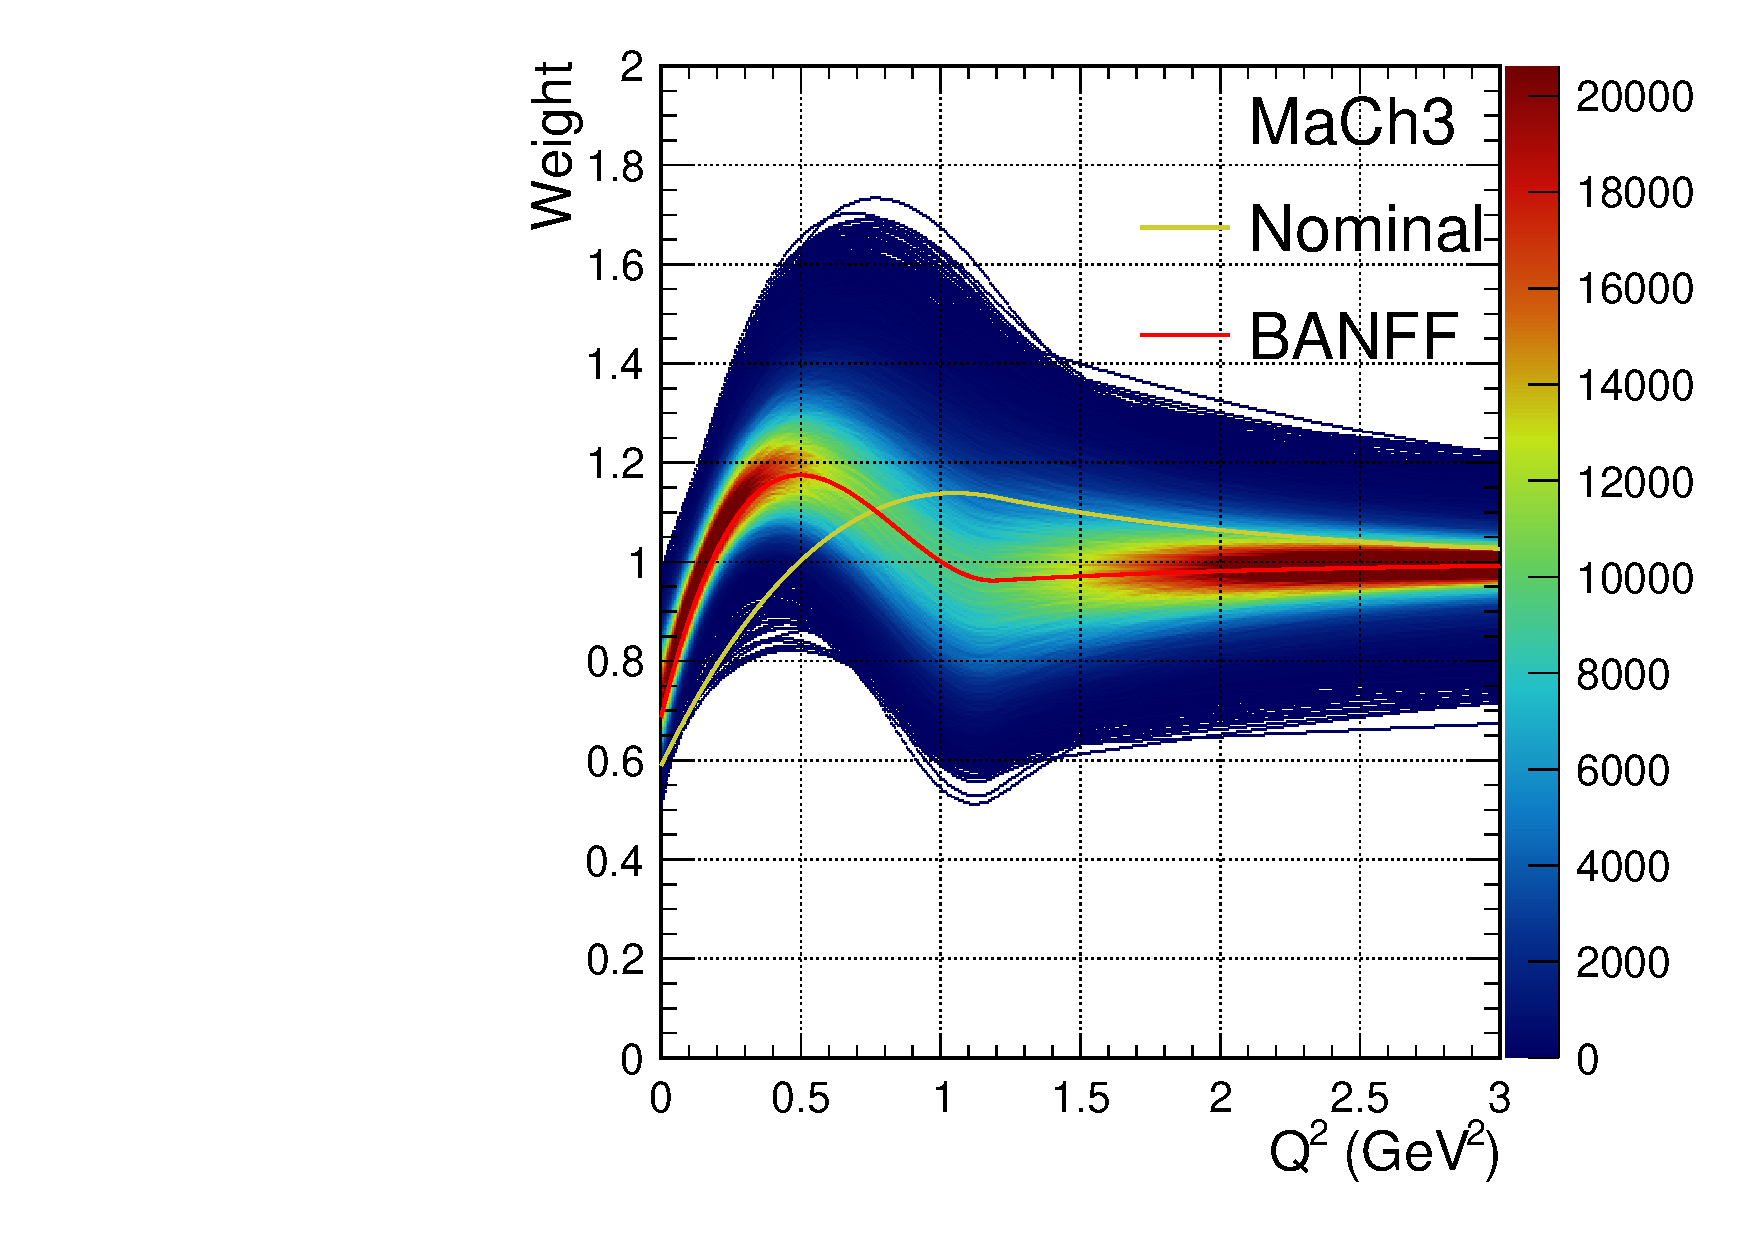
\includegraphics[width=\textwidth, trim={0mm 0mm 0mm 0mm}, clip,page=1]{figures/mach3/data/2017b_NewDet_3Xsec_4Det_5Flux_NewXSecTune_Data_0_BeRPA}
		\caption{Data}
	\end{subfigure}
	\begin{subfigure}[t]{0.49\textwidth}
		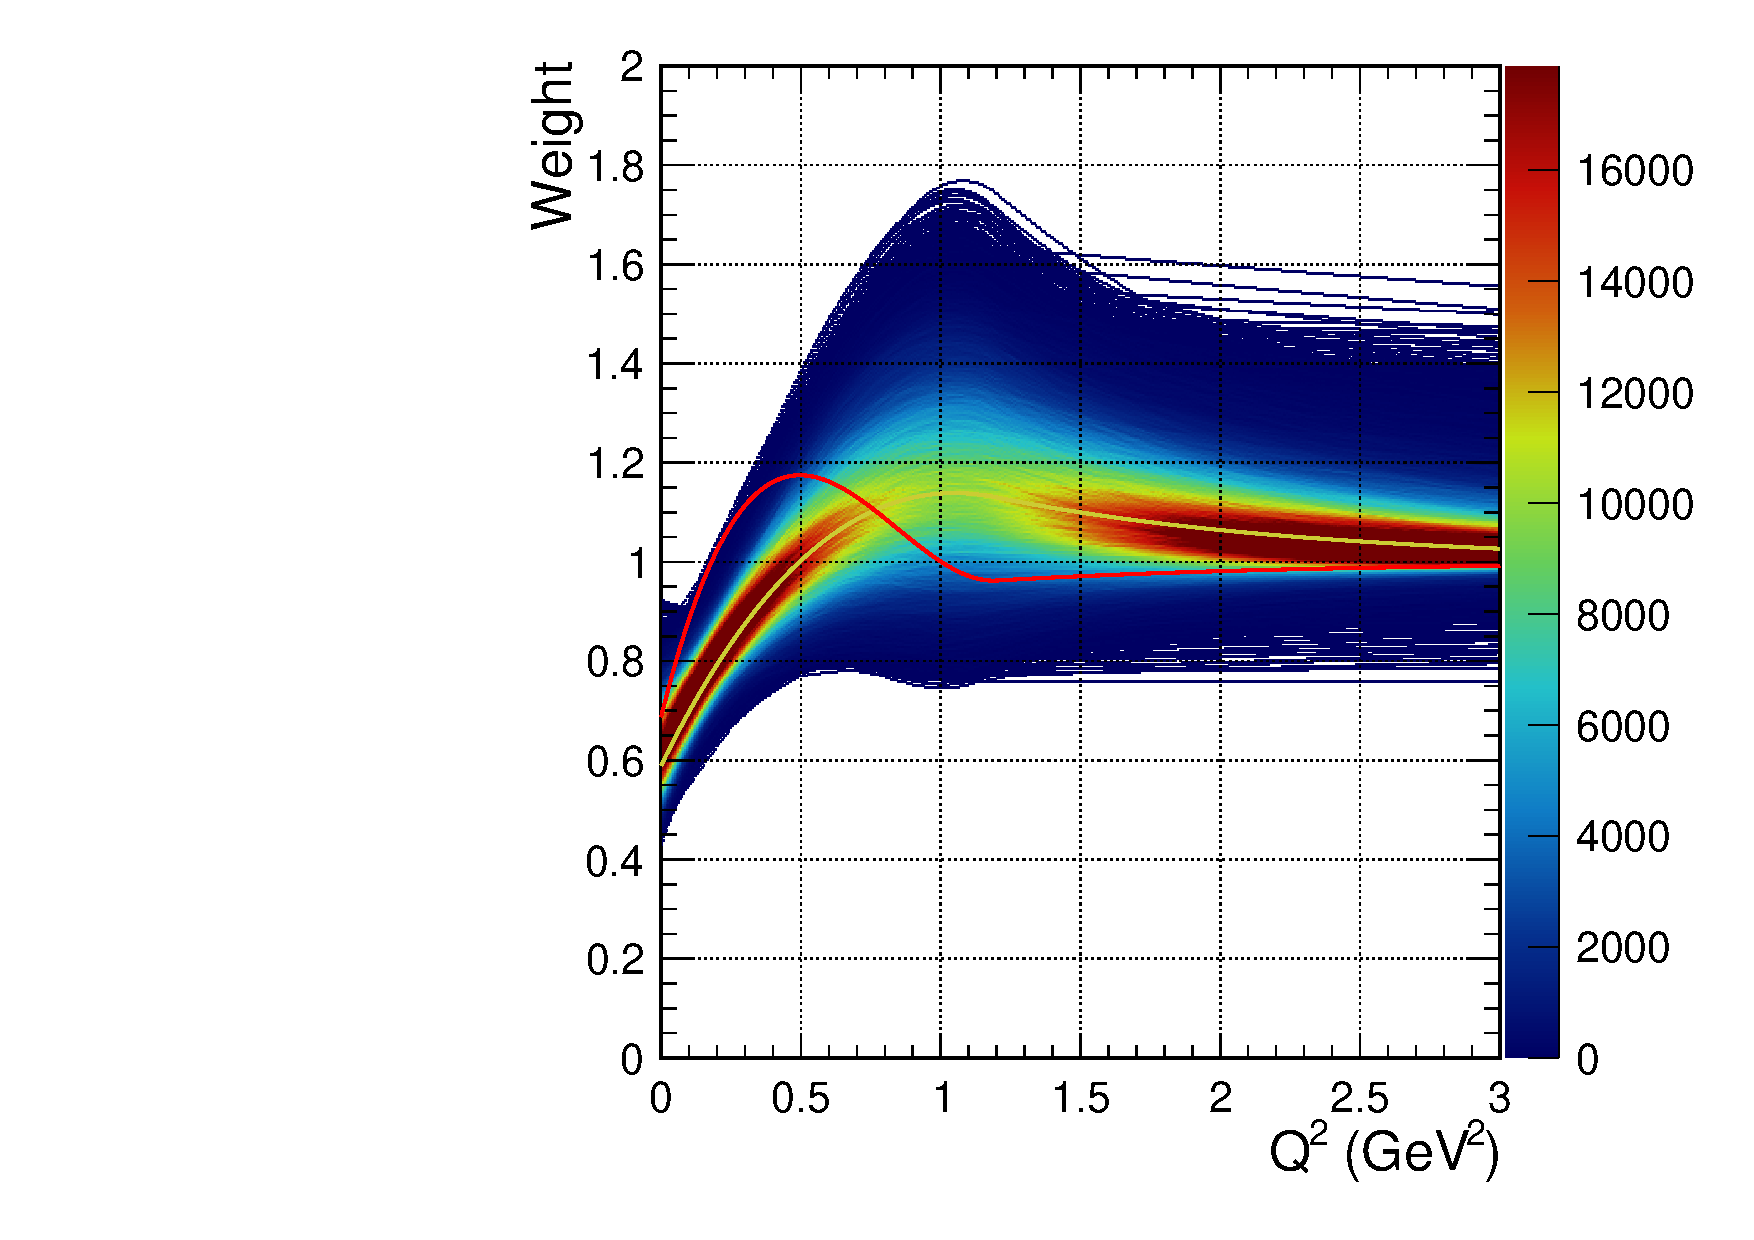
\includegraphics[width=\textwidth, trim={0mm 0mm 0mm 0mm}, clip,page=1]{figures/mach3/data/2017b_NewDet_3Xsec_4Det_5Flux_NewXSecTune_Asimov_0_BeRPA}
		\caption{Asimov}
	\end{subfigure}
\caption{BeRPA weights for each step for the tuned fits to data and Asimov}
\label{fig:berpa_data}
\end{figure}

To understand why BeRPA is heavily distorted from the nominal form, we can look at the $Q^2_{rec}$ distributions of the CC0$\pi$ selections in \autoref{fig:fgd1_cc0pi_q2_berpa} and \autoref{fig:fgd2_cc0pi_q2_berpa}. For both FGD1 and FGD2 we see a clear deficit at low $Q^2$, about 9\% in the first bin. We see the effect of BeRPA A on the pre-fit distributions is to move the low $Q^2$ region specifically, as is the case for BeRPA B although it targets slightly higher $Q^2$. The post-fit distributions are a clear improvement for all of the $Q^2$ space, and this is the driver behind the BeRPA pulls.

\begin{figure}[h]
		\begin{subfigure}[t]{0.49\textwidth}
			\includegraphics[width=\textwidth, trim={0mm 0mm 0mm 6mm}, clip,page=15]{figures/mach3/Asimov/2017b_NewDet_3Xsec_4Det_5Flux_NewXSecTune_Asimov_0_PostFit_5_4_rootstack}
			\caption{Pre-fit, BeRPA A effect}
		\end{subfigure}
		\begin{subfigure}[t]{0.49\textwidth}
			\includegraphics[width=\textwidth, trim={0mm 0mm 0mm 6mm}, clip,page=15]{figures/mach3/data/postfit/2017b_NewData_NewDet_UpdXsecStep_2Xsec_4Det_5Flux_0_PostFit_5_4_rootstack}
			\caption{Post-fit, BeRPA B effect}
		\end{subfigure}
		\caption{FGD1 CC$0\pi$ in $Q^2_{rec}$after the fit to data, showing impact of the BeRPA parameters}
		\label{fig:fgd1_cc0pi_q2_berpa}
\end{figure}

\begin{figure}[h]
	\begin{subfigure}[t]{0.49\textwidth}
		\includegraphics[width=\textwidth, trim={0mm 0mm 0mm 6mm}, clip,page=131]{figures/mach3/Asimov/2017b_NewDet_3Xsec_4Det_5Flux_NewXSecTune_Asimov_0_PostFit_5_4_rootstack}
		\caption{Pre-fit, BeRPA A effect}
	\end{subfigure}
	\begin{subfigure}[t]{0.49\textwidth}
		\includegraphics[width=\textwidth, trim={0mm 0mm 0mm 6mm}, clip,page=127]{figures/mach3/data/postfit/2017b_NewData_NewDet_UpdXsecStep_2Xsec_4Det_5Flux_0_PostFit_5_4_rootstack}
		\caption{Post-fit, BeRPA B effect}
	\end{subfigure}
	\caption{FGD2 CC$0\pi$ in $Q^2_{rec}$ after the fit to data, showing impact of the BeRPA parameters}
	\label{fig:fgd2_cc0pi_q2_berpa}
\end{figure}

Finally we note that the three different MCMC all produced very similar post-fit parameters.

\subsection{Prior predictive}
\label{sec:prior_pred_data}
The prior predictive spectrum and p-values are calculated in the same way as in the fit to Asimov data. Here we expect to see a poor p-value due to the priors' inability to describe ND280 data---the reason behind doing the fit. \autoref{fig:prior_pred_data} shows the prior predictive p-value for all the samples, and as expected not a single parameter variation of the prior model produces a smaller test-statistic against the data than a fluctuation of the prior model does to itself.
\begin{figure}[h]
	\begin{subfigure}[t]{0.49\textwidth}
		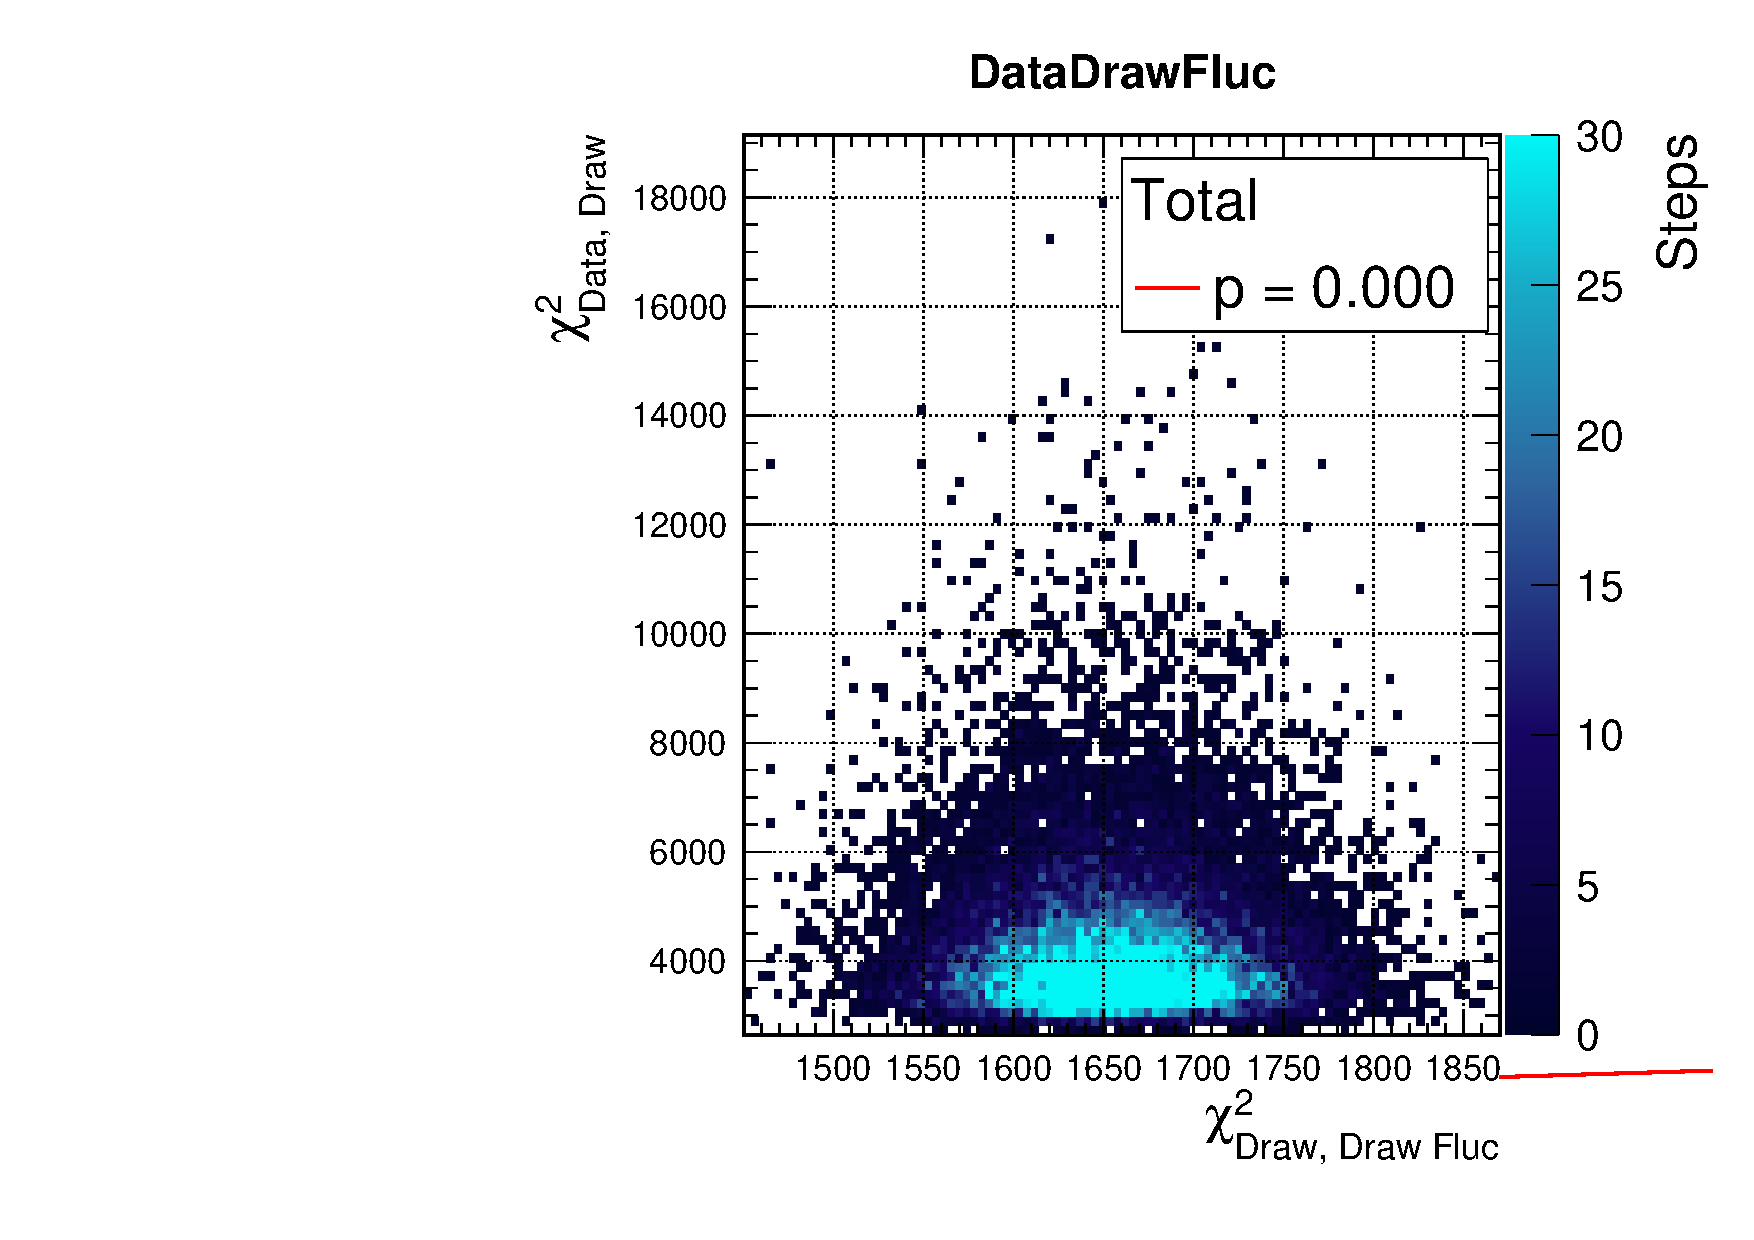
\includegraphics[width=\textwidth, trim={0mm 0mm 0mm 11mm}, clip,page=1]{figures/mach3/data/priorpred/2017b_NewDet_3Xsec_4Det_5Flux_NewXSecTune_Data_merge_PriorPred_procs}
	\end{subfigure}
	\begin{subfigure}[t]{0.49\textwidth}
		\includegraphics[width=\textwidth, trim={0mm 0mm 0mm 11mm}, clip,page=2]{figures/mach3/data/priorpred/2017b_NewDet_3Xsec_4Det_5Flux_NewXSecTune_Data_merge_PriorPred_procs}
	\end{subfigure}
	\caption{Prior predictive spectrum for the data fit}
	\label{fig:prior_pred_data}
\end{figure}

The table of prior predictive p-values broken down by sample is found in \autoref{tab:data_pre_pvalue}. We note the high-statistics FHC samples all consistently having $p=0.000$, and the low-statistics RHC samples having slightly higher p-values than that (maximum of $p=0.017$ for FGD2 CCNTrack \numubar). This is primarily due to statistical fluctuations being a much larger effect for the low-statistics samples compared to the systematic fluctuations.
\begin{table}[h]
	\centering
	\begin{tabular}{l | c c }
		\hline \hline
		Sample & Draw Fluc. & Pred. Fluc. \\
		\hline
		FGD1 0$\pi$ & 0.000 & 0.000 \\
		FGD1 1$\pi$ & 0.000 & 0.000 \\
		FGD1 Other  & 0.000 & 0.000 \\
		\hline
		FGD2 0$\pi$ & 0.000 & 0.000 \\
		FGD2 1$\pi$ & 0.000 & 0.000 \\
		FGD2 Other  & 0.000 & 0.000 \\
		\hline
		FGD1 1Trk & 0.002 & 0.002 \\
		FGD1 NTrk & 0.003 & 0.002 \\
		FGD2 1Trk & 0.001 & 0.000 \\
		FGD2 NTrk & 0.017 & 0.017 \\
		\hline
		FGD1 \numu 1Trk & 0.004 & 0.004 \\
		FGD1 \numu NTrk & 0.011 & 0.009 \\
		FGD2 \numu 1Trk & 0.003 & 0.003 \\
		FGD2 \numu NTrk & 0.003 & 0.003 \\
		\hline
		\hline
	\end{tabular}
	\caption{Prior predictive p-values for each sample after the data fit}
	\label{tab:data_pre_pvalue}
\end{table}

\subsection{Posterior predictive}
\label{sec:post_pred_data}
The posterior predictive spectrum and p-values were calculated in identical way to the Asimov fit, using the model after fitting to data. The resulting test-statistic distribution and p-value is shown in \autoref{fig:posterior_pred_data}, where $p = 0.000$\footnote{A rather discouraging result!}. 
\begin{figure}[h]
	\begin{subfigure}[t]{0.49\textwidth}
		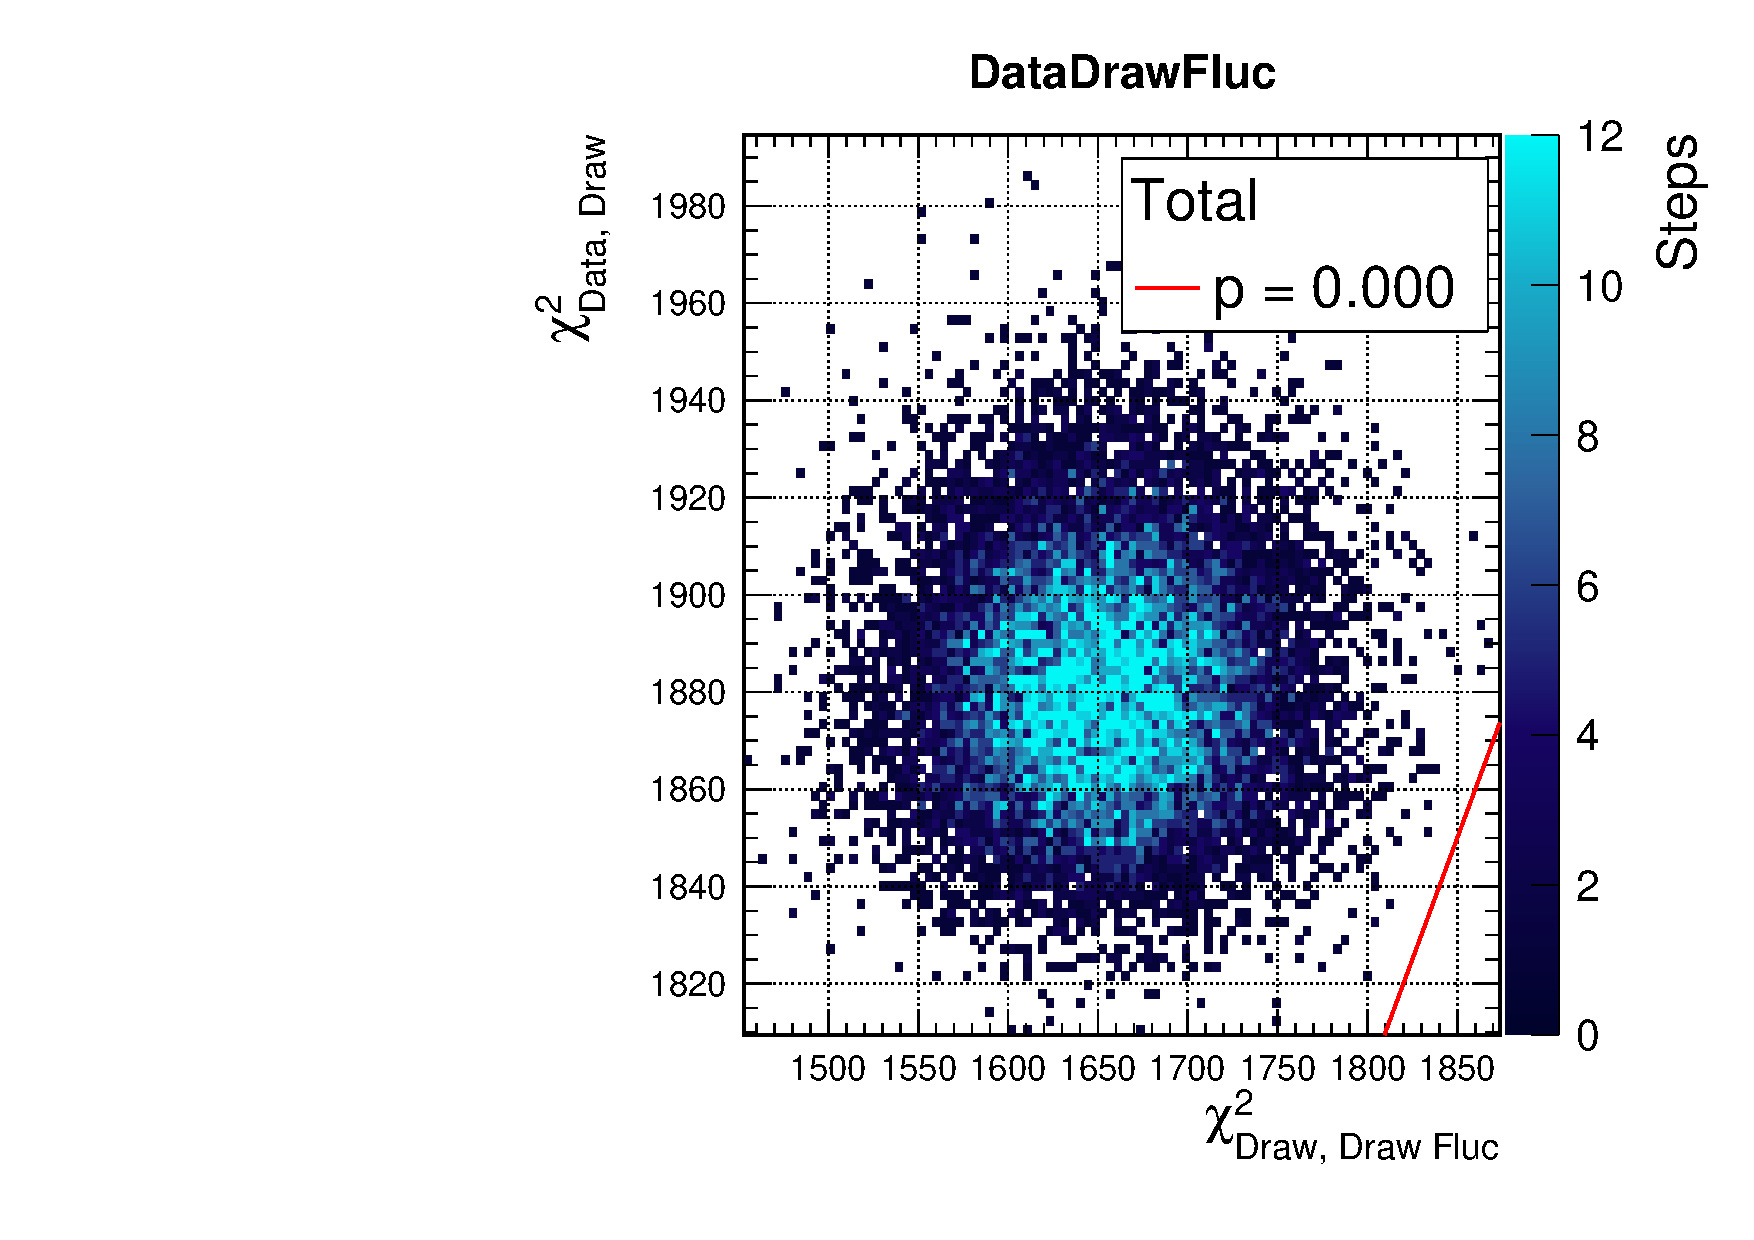
\includegraphics[width=\textwidth, trim={0mm 0mm 0mm 11mm}, clip,page=1]{figures/mach3/data/postpred/2017b_NewData_NewDet_UpdXsecStep_2Xsec_4Det_5Flux_0_PostPred_procs}
	\end{subfigure}
	\begin{subfigure}[t]{0.49\textwidth}
		\includegraphics[width=\textwidth, trim={0mm 0mm 0mm 11mm}, clip,page=2]{figures/mach3/data/postpred/2017b_NewData_NewDet_UpdXsecStep_2Xsec_4Det_5Flux_0_PostPred_procs}
	\end{subfigure}
	\caption{Posterior predictive spectrum for the data fit}
	\label{fig:posterior_pred_data}
\end{figure}

The p-values can further be broken down into sample contributions, and are presented in \autoref{tab:data_post_pvalue}. We note good p-values for all samples except FGD1 CCOther, which is zero. Importantly, the FGD2 CCOther selection observes a good p-value.
\begin{table}[h]
	\centering
\begin{tabular}{l | c c }
	\hline \hline
	Sample & Draw Fluc. & Pred. Fluc. \\
	\hline
	FGD1 0$\pi$ & 0.062 & 0.060 \\
	FGD1 1$\pi$ & 0.078 & 0.075 \\
	\textcolor{red}{FGD1 Other}  & \textcolor{red}{0.000} & \textcolor{red}{0.000} \\
	FGD2 0$\pi$ & 0.115 & 0.114 \\
	FGD2 1$\pi$ & 0.090 & 0.089 \\
	FGD2 Other  & 0.098 & 0.103 \\
	\hline
	FGD1 1Trk & 0.515 & 0.515 \\
	FGD1 NTrk & 0.292 & 0.289 \\
	FGD2 1Trk & 0.265 & 0.260 \\
	FGD2 NTrk & 0.230 & 0.219 \\
	\hline
	FGD1 \numu 1Trk & 0.296 & 0.293 \\
	FGD1 \numu NTrk & 0.842 & 0.839 \\
	FGD2 \numu 1Trk & 0.333 & 0.332 \\
	FGD2 \numu NTrk & 0.587 & 0.591 \\
	\hline
	\hline
\end{tabular}
\caption{Posterior predictive p-values for each sample after the data fit}
\label{tab:data_post_pvalue}
\end{table}

The test-statistic distributions are shown in \autoref{fig:posterior_pred_data_fgd1ccother} with FGD2 as comparison. Whereas the x-axis (statistically fluctuated test-statistic in the model) are similar for the two selections, we see a much higher test-statistic on the y-axis, reflecting the post-fit distribution for FGD1 is much worse than FGD2 and statistical fluctuations of each. This was already hinted at in \autoref{tab:postfit_eventrate}, where FGD1 CCOther showed only a marginal improvement after the fit.

\begin{figure}[h]
	\begin{subfigure}[t]{0.49\textwidth}
		\includegraphics[width=\textwidth, trim={0mm 6mm 0mm 11mm}, clip,page=16]{figures/mach3/data/postpred/2017b_NewData_NewDet_UpdXsecStep_2Xsec_4Det_5Flux_0_PostPred_procs}
	\end{subfigure}
\begin{subfigure}[t]{0.49\textwidth}
	\includegraphics[width=\textwidth, trim={0mm 6mm 0mm 11mm}, clip,page=52]{figures/mach3/data/postpred/2017b_NewData_NewDet_UpdXsecStep_2Xsec_4Det_5Flux_0_PostPred_procs}
\end{subfigure}
	\caption{Bin-by-bin likelihood contributions in \pmu \cosmu for the CCOther selections}
	\label{fig:posterior_pred_data_fgd1ccother}
\end{figure}

\autoref{fig:posterior_pred_data_llh_ccother} shows the likelihood contribution per bin for FGD1 and FGD2 CCOther selections. As expected, there are more bins with high contributions for FGD1 than FGD2 at low $Q^2$, not present in FGD2. For FGD1 CCOther the high likelihood contributions sit primarily at \cosmu=0.9-0.95, whereas FGD2 has it's largest contributions scattered across the phase space.
\begin{figure}[h]
	\begin{subfigure}[t]{0.49\textwidth}
		\includegraphics[width=\textwidth, trim={0mm 6mm 0mm 11mm}, clip,page=21]{figures/mach3/data/postpred/2017b_NewData_NewDet_UpdXsecStep_2Xsec_4Det_5Flux_0_PostPred_procs}
		\caption{FGD1 CCOther}
	\end{subfigure}
	\begin{subfigure}[t]{0.49\textwidth}
		\includegraphics[width=\textwidth, trim={0mm 6mm 0mm 11mm}, clip,page=48]{figures/mach3/data/postpred/2017b_NewData_NewDet_UpdXsecStep_2Xsec_4Det_5Flux_0_PostPred_procs}
		\caption{FGD2 CCOther}
	\end{subfigure}
\caption{Posterior predictive p-values for the two CCOther selections after the data fit}
\label{fig:posterior_pred_data_llh_ccother}
\end{figure}

Inspecting the \pmu \cosmu post-fit distributions in \autoref{fig:postfit_pmucosmu_data_ccother}, the \pmu distributions appear different around 500-1000 MeV, where FGD2 sees a consistent underestimation and FGD1 instead looks statistically fluctuated, slightly above and under 1$\sigma$ from statistics. We also note the effect of the CC DIS parameter being largely a normalisation up to 1.5 GeV. The distributions otherwise look very similar. For the \cosmu projection the two FGDs look very consistent, with the only mild difference at 0.8-0.92, where the bins show opposite behaviour, just outside 1$\sigma$. The CC DIS parameter has the smallest effect in the most forward-going bin.
\begin{figure}[h]
	\begin{subfigure}[t]{\textwidth}
	\begin{subfigure}[t]{0.49\textwidth}
		\includegraphics[width=\textwidth, trim={0mm 0mm 0mm 6mm}, clip,page=101]{figures/mach3/data/postfit/2017b_NewDet_3Xsec_4Det_5Flux_NewXSecTune_Data_merge_PostFit_0_1_rootstack}
	\end{subfigure}
	\begin{subfigure}[t]{0.49\textwidth}
		\includegraphics[width=\textwidth, trim={0mm 0mm 0mm 6mm}, clip,page=102]{figures/mach3/data/postfit/2017b_NewDet_3Xsec_4Det_5Flux_NewXSecTune_Data_merge_PostFit_0_1_rootstack}
	\end{subfigure}
\caption{FGD1 CCOther}
\end{subfigure}
	
\begin{subfigure}[t]{\textwidth}
	\begin{subfigure}[t]{0.49\textwidth}
		\includegraphics[width=\textwidth, trim={0mm 0mm 0mm 6mm}, clip,page=223]{figures/mach3/data/postfit/2017b_NewDet_3Xsec_4Det_5Flux_NewXSecTune_Data_merge_PostFit_0_1_rootstack}
	\end{subfigure}
	\begin{subfigure}[t]{0.49\textwidth}
		\includegraphics[width=\textwidth, trim={0mm 0mm 0mm 6mm}, clip,page=224]{figures/mach3/data/postfit/2017b_NewDet_3Xsec_4Det_5Flux_NewXSecTune_Data_merge_PostFit_0_1_rootstack}
	\end{subfigure}
\caption{FGD2 CCOther}
\end{subfigure}
	\caption{Post-fit distributions for the CCOther selections in \pmu and \cosmu, showing the effect of the CC DIS parameter 1$\sigma$ variation}
	\label{fig:postfit_pmucosmu_data_ccother}
\end{figure}

Projecting the post-fit distributions onto $Q^2_{rec}$ and $E_\nu^{rec}$ in \autoref{fig:postfit_q2enu_data_ccother} the pattern becomes clearer: FGD1 has a consistent under-estimation in the $Q^2_{rec}=0.15-0.4\text{ GeV}^2$ range, whereas FGD2 has a good prediction in all but one bin. Additionally, the CC DIS parameter is almost entirely a normalisation parameter in $Q^2$, so the fit has little freedom in this parameter to change the $Q^2$ shape. Looking at the $E_\nu^{rec}$ distribution we again see mostly consistency across the two FGDs, although FGD1 is underestimated more in the 0.7-0.9 GeV range, approximately within 1$\sigma$ statistical uncertainty.
\begin{figure}[h]
	\begin{subfigure}[t]{\textwidth}
	\begin{subfigure}[t]{0.49\textwidth}
		\includegraphics[width=\textwidth, trim={0mm 0mm 0mm 6mm}, clip,page=97]{figures/mach3/data/postfit/2017b_NewData_NewDet_UpdXsecStep_2Xsec_4Det_5Flux_0_PostFit_5_4_rootstack}
	\end{subfigure}
	\begin{subfigure}[t]{0.49\textwidth}
		\includegraphics[width=\textwidth, trim={0mm 0mm 0mm 6mm}, clip,page=98]{figures/mach3/data/postfit/2017b_NewData_NewDet_UpdXsecStep_2Xsec_4Det_5Flux_0_PostFit_5_4_rootstack}
	\end{subfigure}
\caption{FGD1 CCOther}
\end{subfigure}

\begin{subfigure}[t]{\textwidth}
\begin{subfigure}[t]{0.49\textwidth}
	\includegraphics[width=\textwidth, trim={0mm 0mm 0mm 6mm}, clip,page=219]{figures/mach3/data/postfit/2017b_NewData_NewDet_UpdXsecStep_2Xsec_4Det_5Flux_0_PostFit_5_4_rootstack}
\end{subfigure}
\begin{subfigure}[t]{0.49\textwidth}
	\includegraphics[width=\textwidth, trim={0mm 0mm 0mm 6mm}, clip,page=220]{figures/mach3/data/postfit/2017b_NewData_NewDet_UpdXsecStep_2Xsec_4Det_5Flux_0_PostFit_5_4_rootstack}
\end{subfigure}
\caption{FGD2 CCOther}
\end{subfigure}
	\caption{Post-fit distributions for the CCOther selections in $Q^2_{rec}$ and $E_\nu^{rec}$, showing the effect of the CC DIS parameter 1$\sigma$ variation}
	\label{fig:postfit_q2enu_data_ccother}
\end{figure}

We also look at the more conventional one-dimensional p-values in which we use the posterior or prior predictive spectrum and apply statistical fluctuations in each bin, calculating the test-statistic for each set of fluctuations. 20,000 sets of fluctuations are applied. We then calculate the realised likelihood of the posterior predictive spectrum (``best-fit'') and overlay it on the test-statistic spectrum. For the prior predictive spectrum we name it ``hybrid'' because we're applying fluctuations to predictions of the prior model whereas we're overlaying it with test-statistic of the data vs the posterior predictive model. \autoref{fig:posterior_pred_data_1d} shows the result, in which a good p-value of 0.10 is realised for both methods.

\begin{figure}[h]
	\begin{subfigure}[t]{0.49\textwidth}
		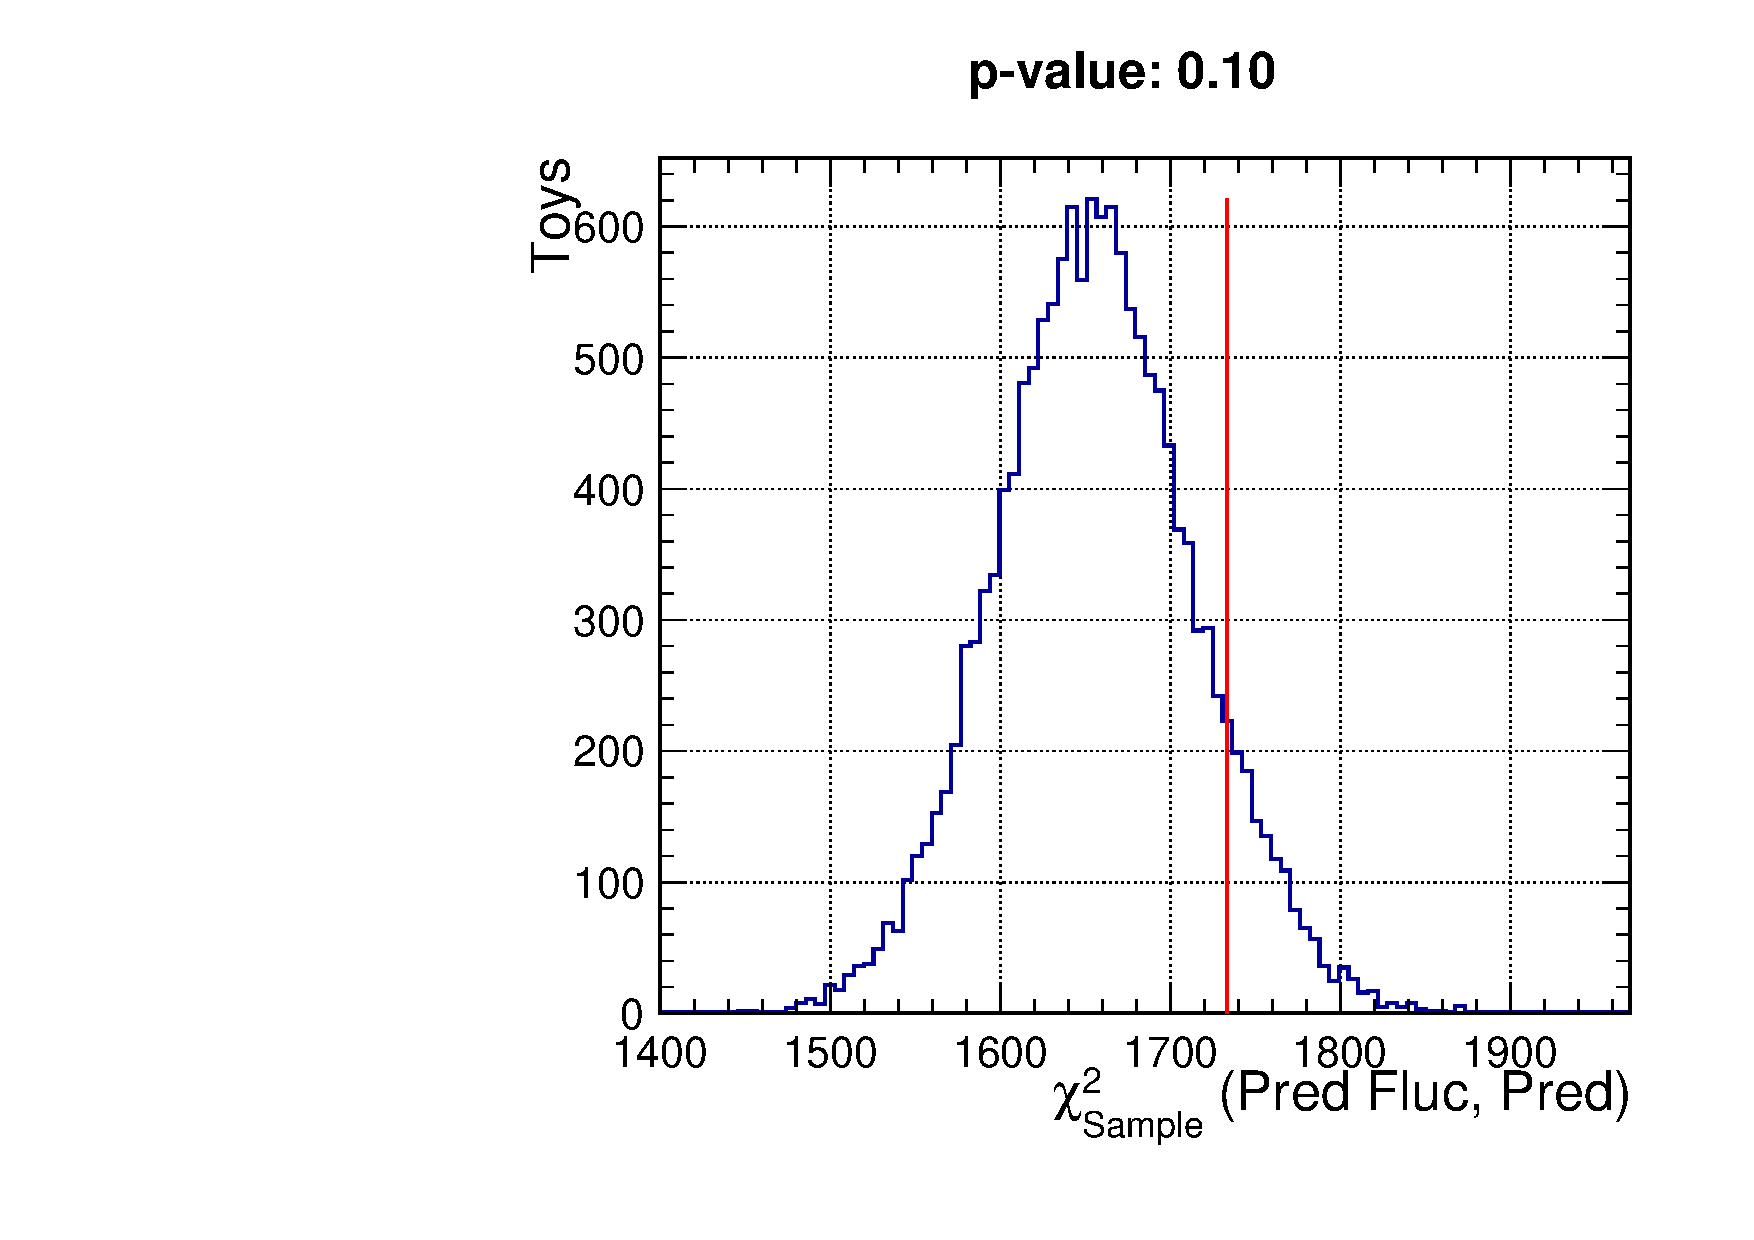
\includegraphics[width=\textwidth, trim={0mm 0mm 0mm 14mm}, clip,page=1]{figures/mach3/data/postpred/postpred_pvalue_1d}
		\caption{Posterior predictive, $p=0.10$}
	\end{subfigure}
	\begin{subfigure}[t]{0.49\textwidth}
		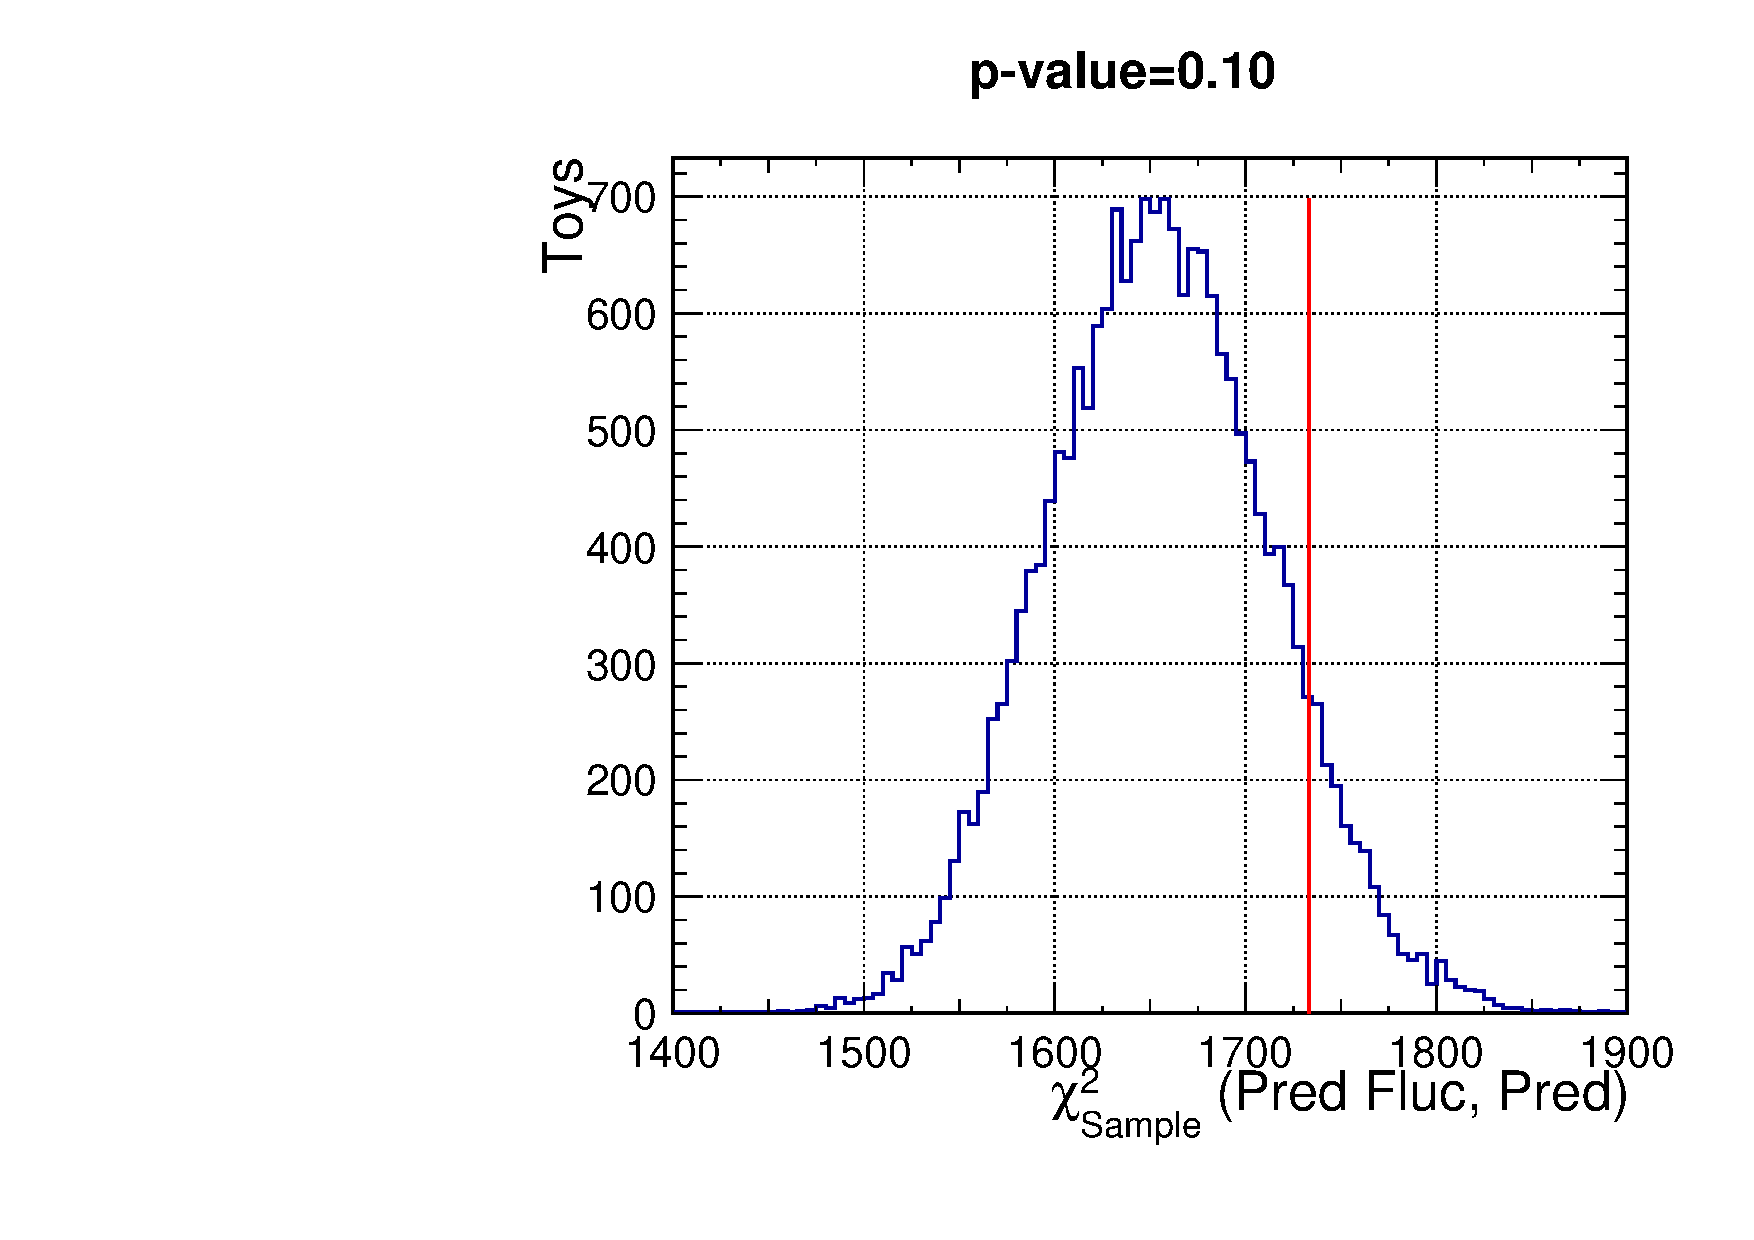
\includegraphics[width=\textwidth, trim={0mm 0mm 0mm 14mm}, clip,page=1]{figures/mach3/data/postpred/PriorPredictive_Hybrid}
		\caption{Prior predictive hybrid, $p=0.10$}
	\end{subfigure}
	\caption{One-dimensional p-value calculations, applying statistical fluctuations}
	\label{fig:posterior_pred_data_1d}
\end{figure}

As we observed a very poor p-value for the two-dimensional calculation in \autoref{tab:data_post_pvalue} the same exercise is repeated looking only at the FGD1 CCOther selection. \autoref{fig:posterior_pred_data_1d_ccother} shows the result for FGD1 CCOther only, using throws from the prior and posterior model for the reference distributions. Although the overall p-value presented in \autoref{fig:posterior_pred_data_1d} is good even though the two-dimensional equivalent was bad, FGD1 CCOther's one-dimensional p-value is still very poor, with the realised test-statistic falling at the very end of the distribution.

\begin{figure}[h]
	\begin{subfigure}[t]{0.49\textwidth}
		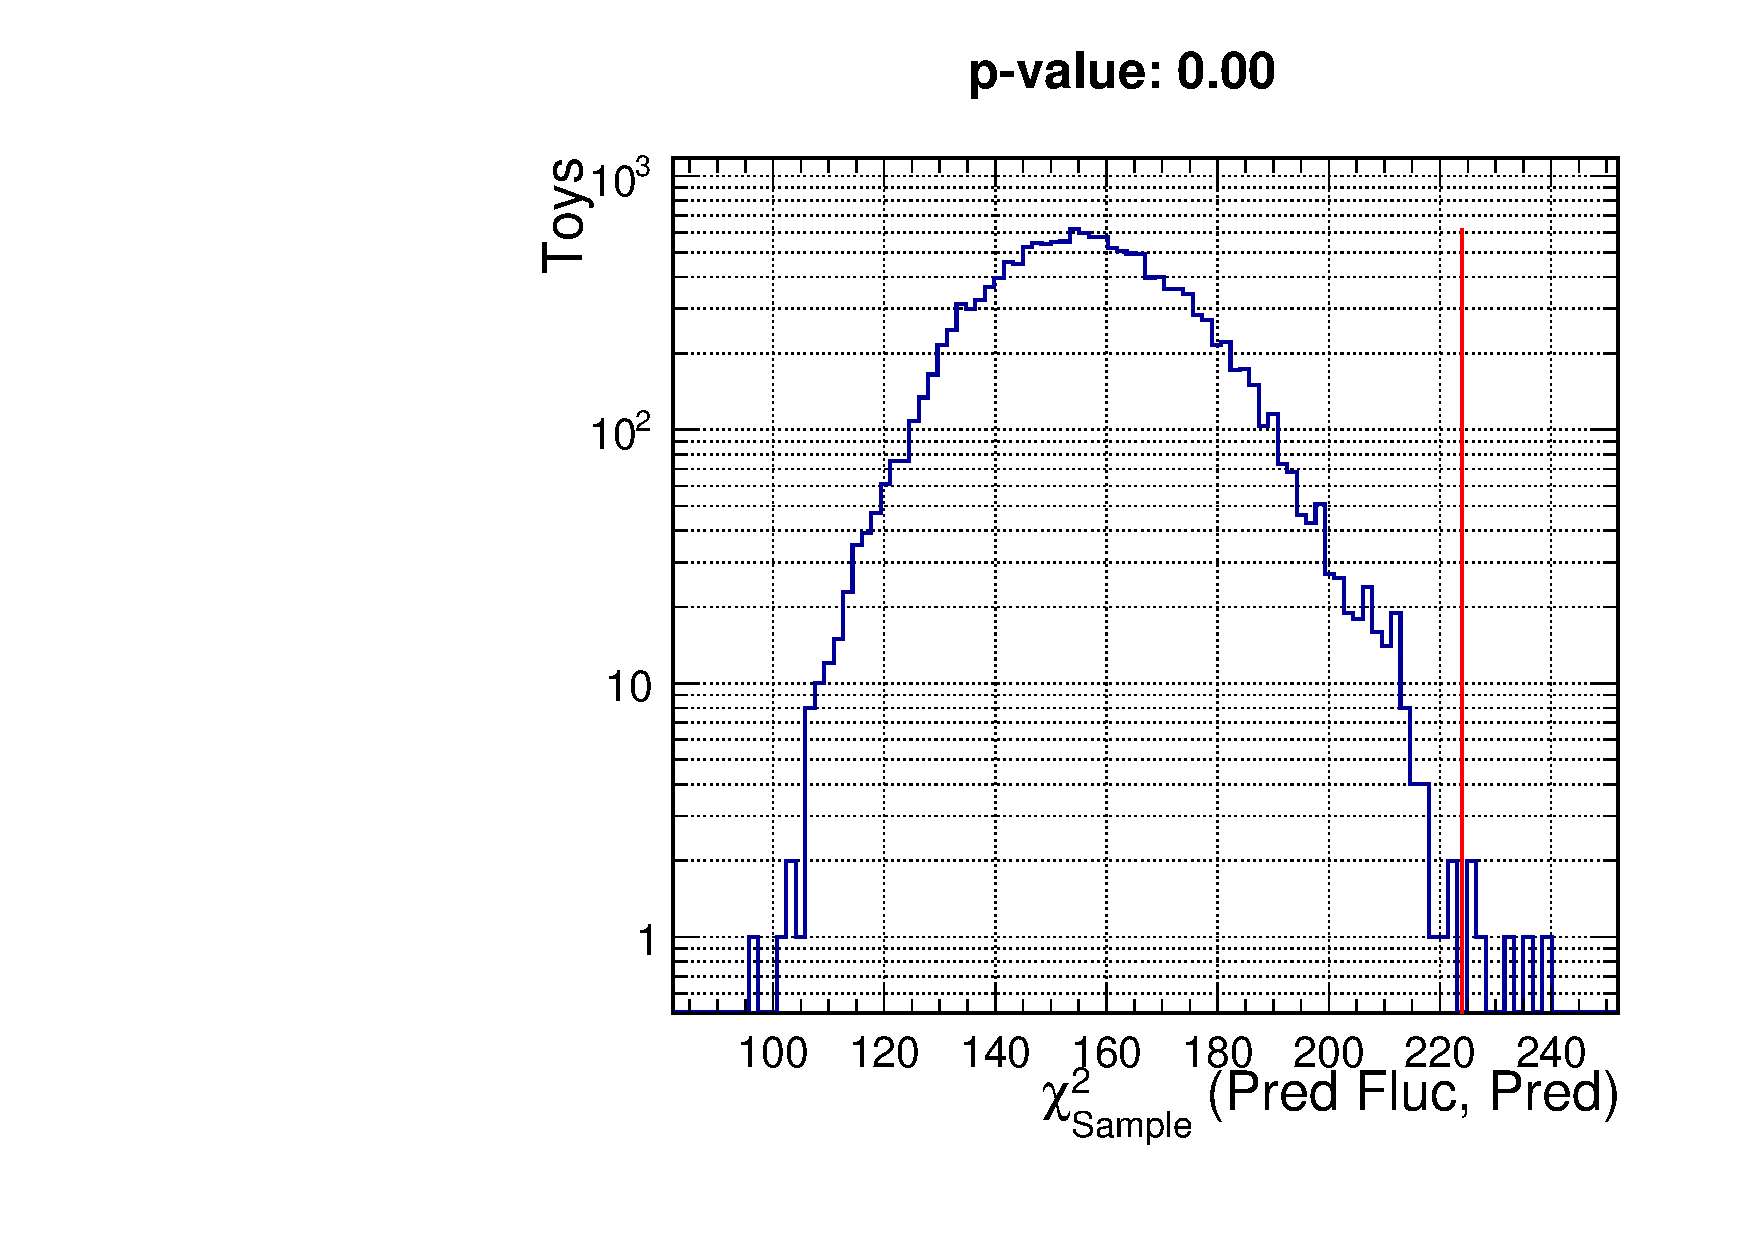
\includegraphics[width=\textwidth, trim={0mm 0mm 0mm 14mm}, clip,page=1]{figures/mach3/data/postpred/pvalue_posteriorpred_fgd1ccother_1d}
		\caption{Posterior predictive, $p=0.00$}
	\end{subfigure}
	\begin{subfigure}[t]{0.49\textwidth}
		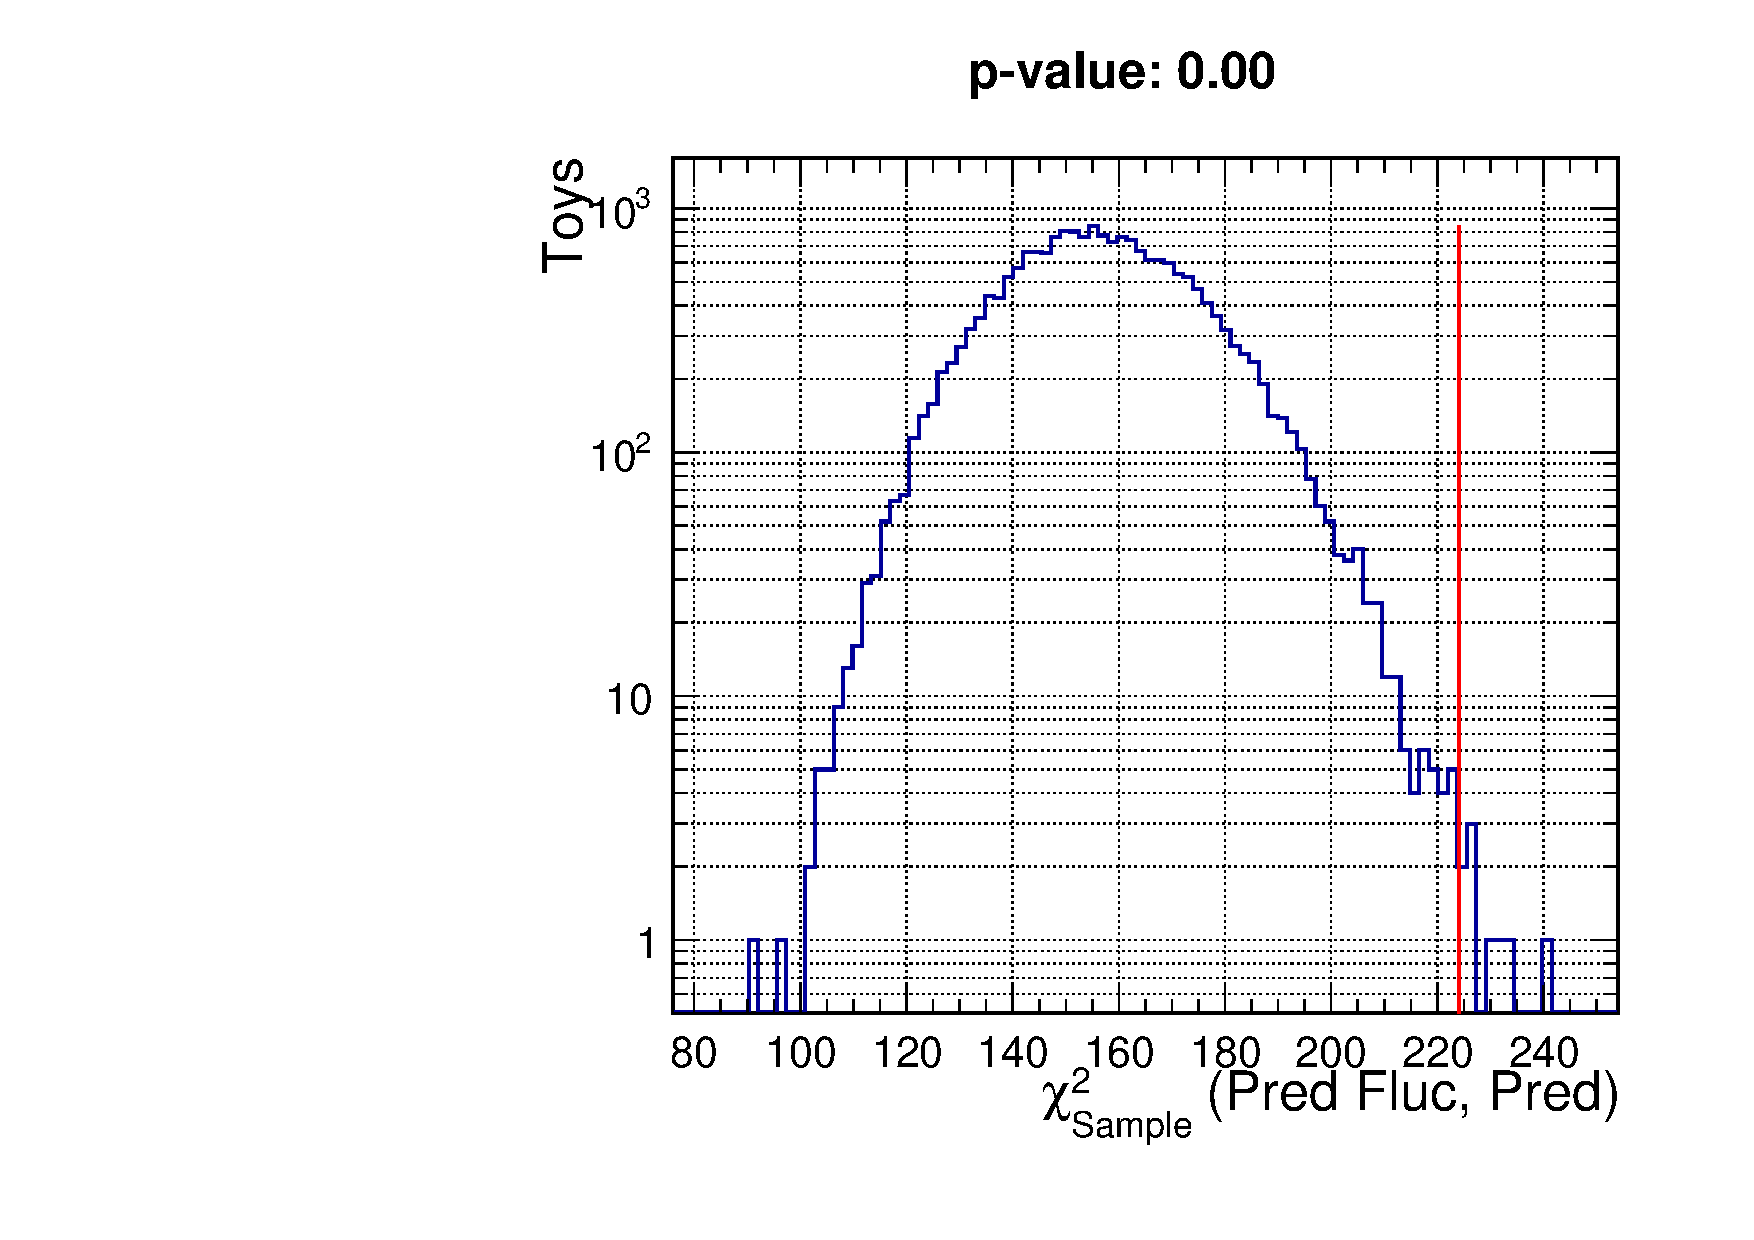
\includegraphics[width=\textwidth, trim={0mm 0mm 0mm 14mm}, clip,page=1]{figures/mach3/data/postpred/prior_pred_fgd1ccother}
		\caption{Prior predictive hybrid, $p=0.00$}
	\end{subfigure}
	\caption{One-dimensional p-value calculations for FGD1 CCOther}
	\label{fig:posterior_pred_data_1d_ccother}
\end{figure}

\subsection{Post-fit distributions}
\autoref{fig:posterior_pred_data_fhc} and \autoref{fig:posterior_pred_data_rhc} shows all the selections' \pmu \cosmu distributions post-fit, using the posterior predictive spectrum as a representation of the post-fit Monte-Carlo. Clearly, the post-fit Monte-Carlo does not describe all distributions, and there is plenty of discrepancies in all selections. The 0$\pi$ and 1Trk selections generally see good predictions post-fit, especially around the flux peak. The 1$\pi$ and Other selections are much patchier and it's difficult to spot patterns in $Q^2$, \pmu or \cosmu. Interestingly, the NTrk predictions are generally better than 1$\pi$ and Other.

\begin{figure}[h]
	\begin{subfigure}[t]{0.32\textwidth}
		\includegraphics[width=\textwidth, trim={20mm 6mm 4mm 11mm}, clip,page=5]{figures/mach3/data/postpred/2017b_NewData_NewDet_UpdXsecStep_2Xsec_4Det_5Flux_0_PostPred_procs}
		\caption{FGD1 0$\pi$}
	\end{subfigure}
	\begin{subfigure}[t]{0.32\textwidth}
		\includegraphics[width=\textwidth, trim={20mm 6mm 4mm 11mm}, clip,page=14]{figures/mach3/data/postpred/2017b_NewData_NewDet_UpdXsecStep_2Xsec_4Det_5Flux_0_PostPred_procs}
		\caption{FGD1 1$\pi$}
	\end{subfigure}
	\begin{subfigure}[t]{0.32\textwidth}
		\includegraphics[width=\textwidth, trim={20mm 6mm 4mm 11mm}, clip,page=23]{figures/mach3/data/postpred/2017b_NewData_NewDet_UpdXsecStep_2Xsec_4Det_5Flux_0_PostPred_procs}
		\caption{FGD1 Other}
	\end{subfigure}

\begin{subfigure}[t]{0.32\textwidth}
	\includegraphics[width=\textwidth, trim={20mm 6mm 4mm 11mm}, clip,page=32]{figures/mach3/data/postpred/2017b_NewData_NewDet_UpdXsecStep_2Xsec_4Det_5Flux_0_PostPred_procs}
	\caption{FGD2 0$\pi$}
\end{subfigure}
\begin{subfigure}[t]{0.32\textwidth}
	\includegraphics[width=\textwidth, trim={20mm 6mm 4mm 11mm}, clip,page=41]{figures/mach3/data/postpred/2017b_NewData_NewDet_UpdXsecStep_2Xsec_4Det_5Flux_0_PostPred_procs}
	\caption{FGD2 1$\pi$}
\end{subfigure}
\begin{subfigure}[t]{0.32\textwidth}
	\includegraphics[width=\textwidth, trim={20mm 6mm 4mm 11mm}, clip,page=50]{figures/mach3/data/postpred/2017b_NewData_NewDet_UpdXsecStep_2Xsec_4Det_5Flux_0_PostPred_procs}
	\caption{FGD2 Other}
\end{subfigure}
\caption{Data to Posterior predictive \pmu \cosmu spectrum ratios after the fit for FHC selections}
\label{fig:posterior_pred_data_fhc}
\end{figure}

\begin{figure}[h]
\begin{subfigure}[t]{0.24\textwidth}
	\includegraphics[width=\textwidth, trim={20mm 6mm 4mm 11mm}, clip,page=59]{figures/mach3/data/postpred/2017b_NewData_NewDet_UpdXsecStep_2Xsec_4Det_5Flux_0_PostPred_procs}
	\caption{FGD1 1Trk}
\end{subfigure}
\begin{subfigure}[t]{0.24\textwidth}
	\includegraphics[width=\textwidth, trim={20mm 6mm 4mm 11mm}, clip,page=68]{figures/mach3/data/postpred/2017b_NewData_NewDet_UpdXsecStep_2Xsec_4Det_5Flux_0_PostPred_procs}
	\caption{FGD1 NTrk}
\end{subfigure}
\begin{subfigure}[t]{0.24\textwidth}
	\includegraphics[width=\textwidth, trim={20mm 6mm 4mm 11mm}, clip,page=77]{figures/mach3/data/postpred/2017b_NewData_NewDet_UpdXsecStep_2Xsec_4Det_5Flux_0_PostPred_procs}
	\caption{FGD2 1Trk}
\end{subfigure}
\begin{subfigure}[t]{0.24\textwidth}
\includegraphics[width=\textwidth, trim={20mm 6mm 4mm 11mm}, clip,page=86]{figures/mach3/data/postpred/2017b_NewData_NewDet_UpdXsecStep_2Xsec_4Det_5Flux_0_PostPred_procs}
\caption{FGD2 NTrk}
\end{subfigure}

\begin{subfigure}[t]{0.24\textwidth}
	\includegraphics[width=\textwidth, trim={20mm 6mm 4mm 11mm}, clip,page=95]{figures/mach3/data/postpred/2017b_NewData_NewDet_UpdXsecStep_2Xsec_4Det_5Flux_0_PostPred_procs}
	\caption{FGD1 \numu 1Trk}
\end{subfigure}
\begin{subfigure}[t]{0.24\textwidth}
	\includegraphics[width=\textwidth, trim={20mm 6mm 4mm 11mm}, clip,page=104]{figures/mach3/data/postpred/2017b_NewData_NewDet_UpdXsecStep_2Xsec_4Det_5Flux_0_PostPred_procs}
	\caption{FGD1 \numu NTrk}
\end{subfigure}
\begin{subfigure}[t]{0.24\textwidth}
	\includegraphics[width=\textwidth, trim={20mm 6mm 4mm 11mm}, clip,page=113]{figures/mach3/data/postpred/2017b_NewData_NewDet_UpdXsecStep_2Xsec_4Det_5Flux_0_PostPred_procs}
	\caption{FGD2 \numu 1Trk}
\end{subfigure}
\begin{subfigure}[t]{0.24\textwidth}
	\includegraphics[width=\textwidth, trim={20mm 6mm 4mm 11mm}, clip,page=122]{figures/mach3/data/postpred/2017b_NewData_NewDet_UpdXsecStep_2Xsec_4Det_5Flux_0_PostPred_procs}
	\caption{FGD1 \numu NTrk}
\end{subfigure}
\caption{Data to Posterior predictive \pmu \cosmu spectrum ratios after the fit for RHC selections}
\label{fig:posterior_pred_data_rhc}
\end{figure}

To better understand the effect of the fit we look at the \pmu and \cosmu distribution before and after the fit. \autoref{fig:fhc_postfit_0pi_1pi} shows the distributions using the prior and posterior predictive spectrum for FGD1 and 2 CC0$\pi$ and CC1$\pi$ selections. 

For CC0$\pi$, we note some tension between FGD1 and FGD2 in the highest \pmu bin for both the prior and posterior predictive distributions where the simulation describes FGD1 well but undershoots FGD2. The post-fit distribution instead fits FGD2 well in this bin and overestimates FGD1. We also note a good improvement in the first two \pmu bins in the post-fit and a large reduction in the error. Moving to the \cosmu distributions, we note little change in the central values of the predictions, where the primary effect appears to be reducing the error band. In \cosmu there seems to be good agreement with FGD1 and FGD2.

For CC1$\pi$, there is acceptable description in \pmu before the fit, except in the first bin. In the 500-100 MeV region we note a consistent over-estimation of the cross-section which gets mostly corrected in the fit. The highest bin is well described for FGD1 and less so for FGD2. Looking at the \cosmu distributions, the pre-fit distribution is much worse, notably in the 0.8-0.98 region and especially present for FGD1. In the post-fit we note most of these corrected, although the 0.8-0.92 region is approximately 1$\sigma$ off.
\begin{figure}[h]
	\begin{subfigure}[t]{\textwidth}
	\begin{subfigure}[t]{0.24\textwidth}
		\includegraphics[width=\textwidth, trim={0mm 0mm 0mm 8mm}, clip,page=10]{figures/mach3/data/priorpred/2017b_NewDet_3Xsec_4Det_5Flux_NewXSecTune_Data_merge_PriorPred_procs}
	\end{subfigure}
	\begin{subfigure}[t]{0.24\textwidth}
		\includegraphics[width=\textwidth, trim={0mm 0mm 0mm 8mm}, clip,page=10]{figures/mach3/data/postpred/2017b_NewData_NewDet_UpdXsecStep_2Xsec_4Det_5Flux_0_PostPred_procs}
	\end{subfigure}
\begin{subfigure}[t]{0.24\textwidth}
\includegraphics[width=\textwidth, trim={0mm 0mm 0mm 8mm}, clip,page=11]{figures/mach3/data/priorpred/2017b_NewDet_3Xsec_4Det_5Flux_NewXSecTune_Data_merge_PriorPred_procs}
\end{subfigure}
	\begin{subfigure}[t]{0.24\textwidth}
		\includegraphics[width=\textwidth, trim={0mm 0mm 0mm 8mm}, clip,page=11]{figures/mach3/data/postpred/2017b_NewData_NewDet_UpdXsecStep_2Xsec_4Det_5Flux_0_PostPred_procs}
	\end{subfigure}
\caption{FGD1 0$\pi$}
\end{subfigure}
	
		\begin{subfigure}[t]{\textwidth}
	\begin{subfigure}[t]{0.24\textwidth}
		\includegraphics[width=\textwidth, trim={0mm 0mm 0mm 8mm}, clip,page=37]{figures/mach3/data/priorpred/2017b_NewDet_3Xsec_4Det_5Flux_NewXSecTune_Data_merge_PriorPred_procs}
	\end{subfigure}
	\begin{subfigure}[t]{0.24\textwidth}
		\includegraphics[width=\textwidth, trim={0mm 0mm 0mm 8mm}, clip,page=37]{figures/mach3/data/postpred/2017b_NewData_NewDet_UpdXsecStep_2Xsec_4Det_5Flux_0_PostPred_procs}
	\end{subfigure}
\begin{subfigure}[t]{0.24\textwidth}
\includegraphics[width=\textwidth, trim={0mm 0mm 0mm 8mm}, clip,page=38]{figures/mach3/data/priorpred/2017b_NewDet_3Xsec_4Det_5Flux_NewXSecTune_Data_merge_PriorPred_procs}
\end{subfigure}
	\begin{subfigure}[t]{0.24\textwidth}
		\includegraphics[width=\textwidth, trim={0mm 0mm 0mm 8mm}, clip,page=38]{figures/mach3/data/postpred/2017b_NewData_NewDet_UpdXsecStep_2Xsec_4Det_5Flux_0_PostPred_procs}
	\end{subfigure}
\caption{FGD2 0$\pi$}
\end{subfigure}
	
	\begin{subfigure}[t]{\textwidth}
	\begin{subfigure}[t]{0.24\textwidth}
		\includegraphics[width=\textwidth, trim={0mm 0mm 0mm 8mm}, clip,page=19]{figures/mach3/data/priorpred/2017b_NewDet_3Xsec_4Det_5Flux_NewXSecTune_Data_merge_PriorPred_procs}
	\end{subfigure}
	\begin{subfigure}[t]{0.24\textwidth}
		\includegraphics[width=\textwidth, trim={0mm 0mm 0mm 8mm}, clip,page=19]{figures/mach3/data/postpred/2017b_NewData_NewDet_UpdXsecStep_2Xsec_4Det_5Flux_0_PostPred_procs}
	\end{subfigure}
\begin{subfigure}[t]{0.24\textwidth}
\includegraphics[width=\textwidth, trim={0mm 0mm 0mm 8mm}, clip,page=20]{figures/mach3/data/priorpred/2017b_NewDet_3Xsec_4Det_5Flux_NewXSecTune_Data_merge_PriorPred_procs}
\end{subfigure}
	\begin{subfigure}[t]{0.24\textwidth}
		\includegraphics[width=\textwidth, trim={0mm 0mm 0mm 8mm}, clip,page=20]{figures/mach3/data/postpred/2017b_NewData_NewDet_UpdXsecStep_2Xsec_4Det_5Flux_0_PostPred_procs}
	\end{subfigure}
\caption{FGD1 1$\pi$}
\end{subfigure}

\begin{subfigure}[t]{\textwidth}
\begin{subfigure}[t]{0.24\textwidth}
	\includegraphics[width=\textwidth, trim={0mm 0mm 0mm 8mm}, clip,page=46]{figures/mach3/data/priorpred/2017b_NewDet_3Xsec_4Det_5Flux_NewXSecTune_Data_merge_PriorPred_procs}
\end{subfigure}
\begin{subfigure}[t]{0.24\textwidth}
	\includegraphics[width=\textwidth, trim={0mm 0mm 0mm 8mm}, clip,page=46]{figures/mach3/data/postpred/2017b_NewData_NewDet_UpdXsecStep_2Xsec_4Det_5Flux_0_PostPred_procs}
\end{subfigure}
\begin{subfigure}[t]{0.24\textwidth}
\includegraphics[width=\textwidth, trim={0mm 0mm 0mm 8mm}, clip,page=47]{figures/mach3/data/priorpred/2017b_NewDet_3Xsec_4Det_5Flux_NewXSecTune_Data_merge_PriorPred_procs}
\end{subfigure}
\begin{subfigure}[t]{0.24\textwidth}
	\includegraphics[width=\textwidth, trim={0mm 0mm 0mm 8mm}, clip,page=47]{figures/mach3/data/postpred/2017b_NewData_NewDet_UpdXsecStep_2Xsec_4Det_5Flux_0_PostPred_procs}
\end{subfigure}
\caption{FGD2 1$\pi$}
\end{subfigure}
\caption{FHC selections \pmu and \cosmu projections before and after fit}
\label{fig:fhc_postfit_0pi_1pi}
\end{figure}

\autoref{fig:fhc_postfit_other} shows the projections for FGD1 and FGD2 CCOther before and after the fit. We note a fairly consistent \pmu distribution between FGD1 and FGD2, which is underestimated around the maximum. The post-fit distribution attempts to correct for this but fluctuations in the data appear present, and it often settles somewhere in between. The \cosmu distributions are only good up until \cosmu=0.85, where the prefit starts to under-estimate the data. We note this under-estimate is present after the fit too, and it appears the freedom in \cosmu is not sufficient to cover the data. 
\begin{figure}[h]
\begin{subfigure}[t]{\textwidth}
\begin{subfigure}[t]{0.24\textwidth}
	\includegraphics[width=\textwidth, trim={0mm 0mm 0mm 8mm}, clip,page=28]{figures/mach3/data/priorpred/2017b_NewDet_3Xsec_4Det_5Flux_NewXSecTune_Data_merge_PriorPred_procs}
\end{subfigure}
\begin{subfigure}[t]{0.24\textwidth}
	\includegraphics[width=\textwidth, trim={0mm 0mm 0mm 8mm}, clip,page=28]{figures/mach3/data/postpred/2017b_NewData_NewDet_UpdXsecStep_2Xsec_4Det_5Flux_0_PostPred_procs}
\end{subfigure}
\begin{subfigure}[t]{0.24\textwidth}
\includegraphics[width=\textwidth, trim={0mm 0mm 0mm 8mm}, clip,page=29]{figures/mach3/data/priorpred/2017b_NewDet_3Xsec_4Det_5Flux_NewXSecTune_Data_merge_PriorPred_procs}
\end{subfigure}
\begin{subfigure}[t]{0.24\textwidth}
	\includegraphics[width=\textwidth, trim={0mm 0mm 0mm 8mm}, clip,page=29]{figures/mach3/data/postpred/2017b_NewData_NewDet_UpdXsecStep_2Xsec_4Det_5Flux_0_PostPred_procs}
\end{subfigure}
\caption{FGD1 Other}
\end{subfigure}

\begin{subfigure}[t]{\textwidth}
\begin{subfigure}[t]{0.24\textwidth}
	\includegraphics[width=\textwidth, trim={0mm 0mm 0mm 8mm}, clip,page=55]{figures/mach3/data/priorpred/2017b_NewDet_3Xsec_4Det_5Flux_NewXSecTune_Data_merge_PriorPred_procs}
\end{subfigure}
\begin{subfigure}[t]{0.24\textwidth}
	\includegraphics[width=\textwidth, trim={0mm 0mm 0mm 8mm}, clip,page=55]{figures/mach3/data/postpred/2017b_NewData_NewDet_UpdXsecStep_2Xsec_4Det_5Flux_0_PostPred_procs}
\end{subfigure}
\begin{subfigure}[t]{0.24\textwidth}
\includegraphics[width=\textwidth, trim={0mm 0mm 0mm 8mm}, clip,page=56]{figures/mach3/data/priorpred/2017b_NewDet_3Xsec_4Det_5Flux_NewXSecTune_Data_merge_PriorPred_procs}
\end{subfigure}
\begin{subfigure}[t]{0.24\textwidth}
	\includegraphics[width=\textwidth, trim={0mm 0mm 0mm 8mm}, clip,page=56]{figures/mach3/data/postpred/2017b_NewData_NewDet_UpdXsecStep_2Xsec_4Det_5Flux_0_PostPred_procs}
\end{subfigure}
\caption{FGD2 Other}
\end{subfigure}
\caption{FHC selections \pmu and \cosmu projections before and after fit}
\label{fig:fhc_postfit_other}
\end{figure}

\autoref{fig:rhc_postfit} shows the RHC \numubar selections for FGD1 and FGD2. For CC1Trk we again note a difference between FGD1 and FGD2 in the highest bin (around 400MeV), which the simulation describes well for FGD2 but not FGD1. Generally the pre-fit description is adequate and the post-fit mostly reduces the error band. The largest difference is around 700 MeV for FGD2, which however is well described for FGD1. For the \cosmu distributions, the pre-fit overestimates FGD1 but well estimates FGD2. The post-fit instead under-estimates FGD2 slightly and well estimates FGD1.

For the CCNTrk distributions the statistics are similar in error to the systematics and the prediction is generally good in \pmu pre-fit and post-fit; again the primary effect of the fit is to reduce the error rather than moving the central value. The \cosmu distribution is similarly well described pre-fit, although the second highest \cosmu bin is overestimated in FGD1 and the highest \cosmu bin is overestimated in FGD2. Post-fit, FGD1 is well described but FGD2 appears consistently over-estimated above \cosmu=0.96, and the highest \cosmu bin is poorly described.
\begin{figure}[h]
	\begin{subfigure}[t]{\textwidth}
	\begin{subfigure}[t]{0.24\textwidth}
		\includegraphics[width=\textwidth, trim={0mm 0mm 0mm 8mm}, clip,page=64]{figures/mach3/data/priorpred/2017b_NewDet_3Xsec_4Det_5Flux_NewXSecTune_Data_merge_PriorPred_procs}
	\end{subfigure}
	\begin{subfigure}[t]{0.24\textwidth}
		\includegraphics[width=\textwidth, trim={0mm 0mm 0mm 8mm}, clip,page=64]{figures/mach3/data/postpred/2017b_NewData_NewDet_UpdXsecStep_2Xsec_4Det_5Flux_0_PostPred_procs}
	\end{subfigure}
\begin{subfigure}[t]{0.24\textwidth}
\includegraphics[width=\textwidth, trim={0mm 0mm 0mm 8mm}, clip,page=65]{figures/mach3/data/priorpred/2017b_NewDet_3Xsec_4Det_5Flux_NewXSecTune_Data_merge_PriorPred_procs}
\end{subfigure}
	\begin{subfigure}[t]{0.24\textwidth}
		\includegraphics[width=\textwidth, trim={0mm 0mm 0mm 8mm}, clip,page=65]{figures/mach3/data/postpred/2017b_NewData_NewDet_UpdXsecStep_2Xsec_4Det_5Flux_0_PostPred_procs}
	\end{subfigure}
\caption{FGD1 1Trk}
\end{subfigure}
	
\begin{subfigure}[t]{\textwidth}
	\begin{subfigure}[t]{0.24\textwidth}
		\includegraphics[width=\textwidth, trim={0mm 0mm 0mm 8mm}, clip,page=82]{figures/mach3/data/priorpred/2017b_NewDet_3Xsec_4Det_5Flux_NewXSecTune_Data_merge_PriorPred_procs}
	\end{subfigure}
	\begin{subfigure}[t]{0.24\textwidth}
		\includegraphics[width=\textwidth, trim={0mm 0mm 0mm 8mm}, clip,page=82]{figures/mach3/data/postpred/2017b_NewData_NewDet_UpdXsecStep_2Xsec_4Det_5Flux_0_PostPred_procs}
	\end{subfigure}
\begin{subfigure}[t]{0.24\textwidth}
\includegraphics[width=\textwidth, trim={0mm 0mm 0mm 8mm}, clip,page=83]{figures/mach3/data/priorpred/2017b_NewDet_3Xsec_4Det_5Flux_NewXSecTune_Data_merge_PriorPred_procs}
\end{subfigure}
	\begin{subfigure}[t]{0.24\textwidth}
		\includegraphics[width=\textwidth, trim={0mm 0mm 0mm 8mm}, clip,page=83]{figures/mach3/data/postpred/2017b_NewData_NewDet_UpdXsecStep_2Xsec_4Det_5Flux_0_PostPred_procs}
	\end{subfigure}
\caption{FGD2 1Trk}
\end{subfigure}
	
\begin{subfigure}[t]{\textwidth}
	\begin{subfigure}[t]{0.24\textwidth}
		\includegraphics[width=\textwidth, trim={0mm 0mm 0mm 8mm}, clip,page=73]{figures/mach3/data/priorpred/2017b_NewDet_3Xsec_4Det_5Flux_NewXSecTune_Data_merge_PriorPred_procs}
	\end{subfigure}
	\begin{subfigure}[t]{0.24\textwidth}
		\includegraphics[width=\textwidth, trim={0mm 0mm 0mm 8mm}, clip,page=73]{figures/mach3/data/postpred/2017b_NewData_NewDet_UpdXsecStep_2Xsec_4Det_5Flux_0_PostPred_procs}
	\end{subfigure}
\begin{subfigure}[t]{0.24\textwidth}
\includegraphics[width=\textwidth, trim={0mm 0mm 0mm 8mm}, clip,page=74]{figures/mach3/data/priorpred/2017b_NewDet_3Xsec_4Det_5Flux_NewXSecTune_Data_merge_PriorPred_procs}
\end{subfigure}
	\begin{subfigure}[t]{0.24\textwidth}
		\includegraphics[width=\textwidth, trim={0mm 0mm 0mm 8mm}, clip,page=74]{figures/mach3/data/postpred/2017b_NewData_NewDet_UpdXsecStep_2Xsec_4Det_5Flux_0_PostPred_procs}
	\end{subfigure}
\caption{FGD1 NTrk}
\end{subfigure}

\begin{subfigure}[t]{\textwidth}
\begin{subfigure}[t]{0.24\textwidth}
	\includegraphics[width=\textwidth, trim={0mm 0mm 0mm 8mm}, clip,page=91]{figures/mach3/data/priorpred/2017b_NewDet_3Xsec_4Det_5Flux_NewXSecTune_Data_merge_PriorPred_procs}
\end{subfigure}
	\begin{subfigure}[t]{0.24\textwidth}
		\includegraphics[width=\textwidth, trim={0mm 0mm 0mm 8mm}, clip,page=91]{figures/mach3/data/postpred/2017b_NewData_NewDet_UpdXsecStep_2Xsec_4Det_5Flux_0_PostPred_procs}
	\end{subfigure}
\begin{subfigure}[t]{0.24\textwidth}
\includegraphics[width=\textwidth, trim={0mm 0mm 0mm 8mm}, clip,page=92]{figures/mach3/data/priorpred/2017b_NewDet_3Xsec_4Det_5Flux_NewXSecTune_Data_merge_PriorPred_procs}
\end{subfigure}
\begin{subfigure}[t]{0.24\textwidth}
\includegraphics[width=\textwidth, trim={0mm 0mm 0mm 8mm}, clip,page=92]{figures/mach3/data/postpred/2017b_NewData_NewDet_UpdXsecStep_2Xsec_4Det_5Flux_0_PostPred_procs}
\end{subfigure}
\caption{FGD2 NTrk}
\end{subfigure}
\caption{RHC \numubar selections \pmu and \cosmu projections before and after fit}
\label{fig:rhc_postfit}
\end{figure}

\autoref{fig:rhc_nu_postfit} shows FGD1 and FGD2 RHC \numu selections, which has comparably low statistics. The 1Trk distributions show good consistency for FGD1 and FGD2. The only large discrepancy is found in the second highest \cosmu bin for FGD1 and the highest \cosmu bin for FGD2. The post-fit fails to correct for this and in general the fit minimises the error band rather than correcting the central values.

For the NTrk distributions we see a similar story: the \pmu distributions are well-described by the prior model and mildly better by the post-fit model. For the \cosmu distribution the most forward-going bins are problematic for both FGD1 and FGD2, which the simulation underestimates strongly.
\begin{figure}[h]
	\begin{subfigure}[t]{\textwidth}
	\begin{subfigure}[t]{0.24\textwidth}
		\includegraphics[width=\textwidth, trim={0mm 0mm 0mm 8mm}, clip,page=100]{figures/mach3/data/priorpred/2017b_NewDet_3Xsec_4Det_5Flux_NewXSecTune_Data_merge_PriorPred_procs}
	\end{subfigure}
	\begin{subfigure}[t]{0.24\textwidth}
		\includegraphics[width=\textwidth, trim={0mm 0mm 0mm 8mm}, clip,page=100]{figures/mach3/data/postpred/2017b_NewData_NewDet_UpdXsecStep_2Xsec_4Det_5Flux_0_PostPred_procs}
	\end{subfigure}
\begin{subfigure}[t]{0.24\textwidth}
\includegraphics[width=\textwidth, trim={0mm 0mm 0mm 8mm}, clip,page=101]{figures/mach3/data/priorpred/2017b_NewDet_3Xsec_4Det_5Flux_NewXSecTune_Data_merge_PriorPred_procs}
\end{subfigure}
	\begin{subfigure}[t]{0.24\textwidth}
		\includegraphics[width=\textwidth, trim={0mm 0mm 0mm 8mm}, clip,page=101]{figures/mach3/data/postpred/2017b_NewData_NewDet_UpdXsecStep_2Xsec_4Det_5Flux_0_PostPred_procs}
	\end{subfigure}
\caption{FGD1 1Trk \numubar}
\end{subfigure}

\begin{subfigure}[t]{\textwidth}
\begin{subfigure}[t]{0.24\textwidth}
	\includegraphics[width=\textwidth, trim={0mm 0mm 0mm 8mm}, clip,page=118]{figures/mach3/data/priorpred/2017b_NewDet_3Xsec_4Det_5Flux_NewXSecTune_Data_merge_PriorPred_procs}
\end{subfigure}
	\begin{subfigure}[t]{0.24\textwidth}
	\includegraphics[width=\textwidth, trim={0mm 0mm 0mm 8mm}, clip,page=118]{figures/mach3/data/postpred/2017b_NewData_NewDet_UpdXsecStep_2Xsec_4Det_5Flux_0_PostPred_procs}
\end{subfigure}
\begin{subfigure}[t]{0.24\textwidth}
\includegraphics[width=\textwidth, trim={0mm 0mm 0mm 8mm}, clip,page=119]{figures/mach3/data/priorpred/2017b_NewDet_3Xsec_4Det_5Flux_NewXSecTune_Data_merge_PriorPred_procs}
\end{subfigure}
\begin{subfigure}[t]{0.24\textwidth}
	\includegraphics[width=\textwidth, trim={0mm 0mm 0mm 8mm}, clip,page=119]{figures/mach3/data/postpred/2017b_NewData_NewDet_UpdXsecStep_2Xsec_4Det_5Flux_0_PostPred_procs}
\end{subfigure}
\caption{FGD2 1Trk \numubar}
\end{subfigure}

\begin{subfigure}[t]{\textwidth}
\begin{subfigure}[t]{0.24\textwidth}
	\includegraphics[width=\textwidth, trim={0mm 0mm 0mm 8mm}, clip,page=109]{figures/mach3/data/priorpred/2017b_NewDet_3Xsec_4Det_5Flux_NewXSecTune_Data_merge_PriorPred_procs}
\end{subfigure}
\begin{subfigure}[t]{0.24\textwidth}
	\includegraphics[width=\textwidth, trim={0mm 0mm 0mm 8mm}, clip,page=109]{figures/mach3/data/postpred/2017b_NewData_NewDet_UpdXsecStep_2Xsec_4Det_5Flux_0_PostPred_procs}
\end{subfigure}
\begin{subfigure}[t]{0.24\textwidth}
\includegraphics[width=\textwidth, trim={0mm 0mm 0mm 8mm}, clip,page=110]{figures/mach3/data/priorpred/2017b_NewDet_3Xsec_4Det_5Flux_NewXSecTune_Data_merge_PriorPred_procs}
\end{subfigure}
\begin{subfigure}[t]{0.24\textwidth}
	\includegraphics[width=\textwidth, trim={0mm 0mm 0mm 8mm}, clip,page=110]{figures/mach3/data/postpred/2017b_NewData_NewDet_UpdXsecStep_2Xsec_4Det_5Flux_0_PostPred_procs}
\end{subfigure}
\caption{FGD1 NTrk \numubar}
\end{subfigure}

\begin{subfigure}[t]{\textwidth}
\begin{subfigure}[t]{0.24\textwidth}
	\includegraphics[width=\textwidth, trim={0mm 0mm 0mm 8mm}, clip,page=127]{figures/mach3/data/priorpred/2017b_NewDet_3Xsec_4Det_5Flux_NewXSecTune_Data_merge_PriorPred_procs}
\end{subfigure}
	\begin{subfigure}[t]{0.24\textwidth}
	\includegraphics[width=\textwidth, trim={0mm 0mm 0mm 8mm}, clip,page=127]{figures/mach3/data/postpred/2017b_NewData_NewDet_UpdXsecStep_2Xsec_4Det_5Flux_0_PostPred_procs}
\end{subfigure}
\begin{subfigure}[t]{0.24\textwidth}
\includegraphics[width=\textwidth, trim={0mm 0mm 0mm 8mm}, clip,page=128]{figures/mach3/data/priorpred/2017b_NewDet_3Xsec_4Det_5Flux_NewXSecTune_Data_merge_PriorPred_procs}
\end{subfigure}
\begin{subfigure}[t]{0.24\textwidth}
	\includegraphics[width=\textwidth, trim={0mm 0mm 0mm 8mm}, clip,page=128]{figures/mach3/data/postpred/2017b_NewData_NewDet_UpdXsecStep_2Xsec_4Det_5Flux_0_PostPred_procs}
\end{subfigure}
\caption{FGD2 NTrk \numubar}
\end{subfigure}
	\caption{RHC \numu selections \pmu and \cosmu projections before and after fit}
	\label{fig:rhc_nu_postfit}
\end{figure}

\subsection{Covariance matrix}
\label{sec:covariance_data}
\autoref{fig:postfit_corr_nd280} shows the post-fit covariance matrix for the ND280 parameters, directly comparable to \autoref{fig:asimov_nd_corr}. The bottom row shows the absolute difference in each matrix multiplied by the sign of each matrix. Blue entries have flipped sign, whereas red entries have kept their sign in the fit to Asimov and real data. We see the flux parameters never flip signs and generally the covariance barely changes, whereas the correlation changes at a maximum of $\sim0.2$. The only parameters that swap signs are the cross-section parameters. Although sometimes strong in the correlation plot, looking at the covariance plot we see the effects are often limited to weak changes in the covariances.

For the cross-section parameters we note stronger correlations for the dominant 2p2h parameters (2p2h shape C and 2p2h norm $\nu$) and the flux parameters. Whereas the 2p2p normalisation correlates stronger, the 2p2h shape parameter swaps sign frequently. This may be a result of the parameter being pushed against the boundary in the data fit. Interestingly, 2p2h norm $\nu$ correlations very differently with BeRPA A: we swap the sign and the strength. Again this is not surprising: the BeRPA A parameter is pulled far from the value in the Asimov fit (the prior), so is entirely possible to correlate differently.

Looking purely at the correlations, there are strong relations between $M_A^{QE}$, 2p2h normalisations, BeRPA A, BeRPA B, $C_5^A$, CC DIS, NC other and the flux parameters, and don't flip signs to the Asimov case. $M_A^{QE}$ correlates strongly with BeRPA A, B and D as expected from their parametrisations (both being approximately $Q^2$ shape variations for CCQE interactions). The correlation with the flux parameters is due to ND280 data sitting in a relatively small $E_\nu, Q^2$ region, correlating heavily with $E_\nu$ normalisations up to 1 GeV (in turn correlating with the other flux parameters due to the internal flux parameter correlations). The 2p2h normalisations contribute a relatively large portion to the CC0$\pi$ sample across $E_\nu$, giving rise to that correlation. For the same reason, the $C_5^A$ correlations enters due to the parameter controlling the normalisation of one of the interaction terms in the single pion model\red{insert reference?}. Finally the CC DIS parameter is parametrised as $0.4/E_\nu$ for DIS events, so directly correlates to any other parameters that are dependent on $E_\nu$, such as the flux parameters.

\red{talk more here?}
\begin{figure}[h]
\begin{subfigure}[t]{\textwidth}
	\begin{subfigure}[t]{0.49\textwidth}
		\includegraphics[width=\textwidth, trim={0mm 0mm 0mm 0mm}, clip,page=5]{figures/mach3/data/corr/2017b_NewData_NewDet_UpdXsecStep_2Xsec_4Det_5Flux_0_drawCorr}
	\end{subfigure}
	\begin{subfigure}[t]{0.49\textwidth}
		\includegraphics[width=\textwidth, trim={0mm 0mm 0mm 0mm}, clip,page=6]{figures/mach3/data/corr/2017b_NewData_NewDet_UpdXsecStep_2Xsec_4Det_5Flux_0_drawCorr}
	\end{subfigure}
\caption{$\sqrt{V_{i,j}}$ and correlation matrices}
\end{subfigure}

\begin{subfigure}[t]{\textwidth}
	\begin{subfigure}[t]{0.49\textwidth}
		\includegraphics[width=\textwidth, trim={0mm 0mm 0mm 0mm}, clip,page=1]{figures/mach3/data/corr/data_asimov_corr_ratio}
	\end{subfigure}
	\begin{subfigure}[t]{0.49\textwidth}
		\includegraphics[width=\textwidth, trim={0mm 0mm 0mm 0mm}, clip,page=2]{figures/mach3/data/corr/data_asimov_corr_ratio}
	\end{subfigure}
	\caption{Asimov/Data for the $\sqrt{V_{i,j}}$ and correlation matrices}
\end{subfigure}
\caption{Post-fit covariance matrix for the data fit, showing ND280 parameters}
\label{fig:postfit_corr_nd280}
\end{figure}


%\autoref{fig:postfit_corr_flux}
%\begin{figure}[h]
%	\begin{subfigure}[t]{0.49\textwidth}
%		\includegraphics[width=\textwidth, trim={0mm 0mm 0mm 0mm}, clip,page=8]{figures/mach3/data/corr/2017b_NewData_NewDet_UpdXsecStep_2Xsec_4Det_5Flux_0_drawCorr}
%	\end{subfigure}
%	\begin{subfigure}[t]{0.49\textwidth}
%		\includegraphics[width=\textwidth, trim={0mm 0mm 0mm 0mm}, clip,page=9]{figures/mach3/data/corr/2017b_NewData_NewDet_UpdXsecStep_2Xsec_4Det_5Flux_0_drawCorr}
%	\end{subfigure}
%	\caption{Post-fit covariance matrix for the data fit, showing the flux parameters}
%	\label{fig:postfit_corr_flux}
%\end{figure}


%\autoref{fig:postfit_corr_xsec}
%\begin{figure}[h]
%	\begin{subfigure}[t]{0.49\textwidth}
%		\includegraphics[width=\textwidth, trim={0mm 0mm 0mm 0mm}, clip,page=11]{figures/mach3/data/corr/2017b_NewData_NewDet_UpdXsecStep_2Xsec_4Det_5Flux_0_drawCorr}
%	\end{subfigure}
%	\begin{subfigure}[t]{0.49\textwidth}
%		\includegraphics[width=\textwidth, trim={0mm 0mm 0mm 0mm}, clip,page=12]{figures/mach3/data/corr/2017b_NewData_NewDet_UpdXsecStep_2Xsec_4Det_5Flux_0_drawCorr}
%	\end{subfigure}
%	\caption{Post-fit covariance matrix for the data fit, showing the interaction parameters}
%	\label{fig:postfit_corr_xsec}
%\end{figure}

\subsection{Alternate studies}
\label{sec:data_alt_studies}
The largest concern for the analysis presented was the poor posterior predictive p-value, driven primarily by the modelling of the FGD1 CCOther selection. A number of compatibility studies were made to study the effects of this and various other model choices, e.g. using BeRPA and 2p2h shape.

%\subsubsection{Mirrored 2p2h splines}
%Finished but don't include

\subsubsection{Neutrino vs anti-neutrino}
The data-sets used for the full fit (runs 2 to 6) spanned neutrino (runs 2 to 4) and anti-neutrino runs (runs 5 to 6), as shown in  \autoref{tab:pot_2017}. As seen in the table, the FHC/RHC ratio is roughly 1.5 and looking at \autoref{tab:event_rates_2017} the FHC/RHC event rate ratio is 3.4. Hence the full run 2 to 6 fit is dominated by FHC running and hence by neutrino rather than anti-neutrino interactions.

To investigate the compatibility between neutrino and anti-neutrino data at T2K, we perform data fits to run 2 to 4 data and to run 5 to 6 data separately, comparing results to the full fit. Due to the different event rates we expect larger constraints on parameters from the FHC data (run 2 to 4) than the RHC data (run 5 to 6), and the overall constraint from the full fit to come primarily from the FHC data. 

\autoref{fig:flux_data_nd280_nuvsnubar} shows the ND280 flux parameters after the fit with the prefit uncertainty band in red. As expected, the anti-neutrino fit barely moves the central values for the FHC parameters, and the small movements are due to the covariance matrix penalty tying the FHC and RHC flux together. The full fit often settles between the two separate fits' central values, but in cases of extreme pulls the full fit sits closer to the neutrino fit. The neutrino-only fit pulls the extreme cases a little further (e.g. e.g. FHC \numu $\sim1\text{ GeV}$, high $E_\nu$ \numu and \numubar), highlighting the slight tension with the prior covariance matrix. Generally the flux parameters are compatible throughout and often well within $1\sigma$ of each other.
\begin{figure}[h]
	\begin{subfigure}[t]{0.10\textwidth}
		\includegraphics[width=\textwidth, trim={0mm 0mm 0mm 0mm}, clip,page=1]{figures/mach3/data/alt/2017b_Run2to4_Data_merge_2017b_Run56_Data_merge_2017b_NewData_NewDet_UpdXsecStep_2Xsec_4Det_5Flux_0}
	\end{subfigure}
	
	\begin{subfigure}[t]{0.24\textwidth}
		\includegraphics[width=\textwidth, trim={0mm 0mm 0mm 0mm}, clip,page=2]{figures/mach3/data/alt/2017b_Run2to4_Data_merge_2017b_Run56_Data_merge_2017b_NewData_NewDet_UpdXsecStep_2Xsec_4Det_5Flux_0}
	\end{subfigure}
	\begin{subfigure}[t]{0.24\textwidth}
		\includegraphics[width=\textwidth, trim={0mm 0mm 0mm 0mm}, clip,page=3]{figures/mach3/data/alt/2017b_Run2to4_Data_merge_2017b_Run56_Data_merge_2017b_NewData_NewDet_UpdXsecStep_2Xsec_4Det_5Flux_0}
	\end{subfigure}
	\begin{subfigure}[t]{0.24\textwidth}
		\includegraphics[width=\textwidth, trim={0mm 0mm 0mm 0mm}, clip,page=4]{figures/mach3/data/alt/2017b_Run2to4_Data_merge_2017b_Run56_Data_merge_2017b_NewData_NewDet_UpdXsecStep_2Xsec_4Det_5Flux_0}
	\end{subfigure}
	\begin{subfigure}[t]{0.24\textwidth}
		\includegraphics[width=\textwidth, trim={0mm 0mm 0mm 0mm}, clip,page=5]{figures/mach3/data/alt/2017b_Run2to4_Data_merge_2017b_Run56_Data_merge_2017b_NewData_NewDet_UpdXsecStep_2Xsec_4Det_5Flux_0}
	\end{subfigure}
	
	\begin{subfigure}[t]{0.24\textwidth}
		\includegraphics[width=\textwidth, trim={0mm 0mm 0mm 0mm}, clip,page=6]{figures/mach3/data/alt/2017b_Run2to4_Data_merge_2017b_Run56_Data_merge_2017b_NewData_NewDet_UpdXsecStep_2Xsec_4Det_5Flux_0}
	\end{subfigure}
	\begin{subfigure}[t]{0.24\textwidth}
		\includegraphics[width=\textwidth, trim={0mm 0mm 0mm 0mm}, clip,page=7]{figures/mach3/data/alt/2017b_Run2to4_Data_merge_2017b_Run56_Data_merge_2017b_NewData_NewDet_UpdXsecStep_2Xsec_4Det_5Flux_0}
	\end{subfigure}
	\begin{subfigure}[t]{0.24\textwidth}
		\includegraphics[width=\textwidth, trim={0mm 0mm 0mm 0mm}, clip,page=8]{figures/mach3/data/alt/2017b_Run2to4_Data_merge_2017b_Run56_Data_merge_2017b_NewData_NewDet_UpdXsecStep_2Xsec_4Det_5Flux_0}
	\end{subfigure}
	\begin{subfigure}[t]{0.24\textwidth}
		\includegraphics[width=\textwidth, trim={0mm 0mm 0mm 0mm}, clip,page=9]{figures/mach3/data/alt/2017b_Run2to4_Data_merge_2017b_Run56_Data_merge_2017b_NewData_NewDet_UpdXsecStep_2Xsec_4Det_5Flux_0}
	\end{subfigure}
	\caption{ND280 flux parameters after the data fit for different run periods}
	\label{fig:flux_data_nd280_nuvsnubar}
\end{figure}

\autoref{fig:xsec_data_nuvsnubar} shows the interaction parameters where we see more movement than for the flux parameters. As expected, the FHC fit doesn't constrain the $\bar{\nu}$ parameters, such as 2p2h norm $\bar{\nu}$, and the RHC fit barely constrains the $\nu$ parameters (only through the \numu in RHC samples). Generally the RHC fit results are closer to the prior values, largely due to the smaller statistics. Where the FHC fit pulls strongly (e.g. 2p2h shape at boundary, very high BeRPA B, $I_{1/2}$ background), the RHC fit generally sits inside the 1$\sigma$ band instead. 

Interestingly, the 2p2h norm $\bar{\nu}$ parameter is fitted higher in the RHC fit than it is in the joint fit, likely due to correlations with the flux parameters. We also note a smaller $M_A^{QE}$ value for the anti-neutrino fit ($M_A^{QE} = 1.04\pm0.12 \text{ GeV}$), almost identical to the bubble chamber value. The larger tensions are present in the single-pion parameters, where the two fits seem to pull $M_A^{RES}$ and $I_{1/2}$ in opposite directions from the central value. Again, the RHC fit barely has enough statistics to pull 1$\sigma$ from the prior, and more data is likely needed to draw conclusions.
\begin{figure}[h]
	\begin{subfigure}[t]{0.49\textwidth}
		\includegraphics[width=\textwidth, trim={0mm 0mm 0mm 0mm}, clip,page=18]{figures/mach3/data/alt/2017b_Run2to4_Data_merge_2017b_Run56_Data_merge_2017b_NewData_NewDet_UpdXsecStep_2Xsec_4Det_5Flux_0}
	\end{subfigure}
	\begin{subfigure}[t]{0.49\textwidth}
		\includegraphics[width=\textwidth, trim={0mm 0mm 0mm 0mm}, clip,page=19]{figures/mach3/data/alt/2017b_Run2to4_Data_merge_2017b_Run56_Data_merge_2017b_NewData_NewDet_UpdXsecStep_2Xsec_4Det_5Flux_0}
	\end{subfigure}
	
	\begin{subfigure}[t]{0.49\textwidth}
		\includegraphics[width=\textwidth, trim={0mm 0mm 0mm 0mm}, clip,page=20]{figures/mach3/data/alt/2017b_Run2to4_Data_merge_2017b_Run56_Data_merge_2017b_NewData_NewDet_UpdXsecStep_2Xsec_4Det_5Flux_0}
	\end{subfigure}
	\begin{subfigure}[t]{0.49\textwidth}
		\includegraphics[width=\textwidth, trim={0mm 0mm 0mm 0mm}, clip,page=21]{figures/mach3/data/alt/2017b_Run2to4_Data_merge_2017b_Run56_Data_merge_2017b_NewData_NewDet_UpdXsecStep_2Xsec_4Det_5Flux_0}
	\end{subfigure}
	\caption{Interaction parameters after the data fit for different run periods}
	\label{fig:xsec_data_nuvsnubar}
\end{figure}

In conclusion, the comparisons suggests there are some tensions between neutrino and anti-neutrino data fits, with the anti-neutrino fits often favouring a best-fit closer to the central value. However this is largely due to the weaker constraint from the sample likelihood due to the lower statistics, making the prior likelihood contribution more important.

\subsubsection{FGD1 vs FGD2}
Reading off \autoref{tab:event_rates_2017} the ratio of FGD1 to FGD2 data is roughly 1, as expected from the detector design. The target in FGD1 is plastic scintillator ($C_8H_8$), whereas FGD2 is alternating layers plastic scintillator and passive water layers. Hence the constraints on $H_2O$ related parameters (e.g. 2p2h shape O) comes purely from FGD2. The location of the TPCs relative each FGD is also important from the view of reconstruction and related systematics: the PID for forward-going tracks is much better in FGD1 due to the two downstream TPCs, whereas FGD2 generally has better backwards going tracking capabilities due to the two upstream TPCs.

\autoref{fig:flux_data_nd280_fdg1vsfgd2} shows the ND280 flux parameters after the fit, in which we mostly similar results for the dominant parameters (correct-sign \numu and \nue). The largest differences happen above $E_\nu=3\text{ GeV}$, where the two fits diverge: FGD2 favouring a much lower flux normalisation at higher energies. The full fit then settles roughtly in between the two fits with an uncertainty covering each individual FGD fit's extreme 1$\sigma$ uncertainty. Interestingly, FGD2 prefers a nominal flux weight at higher $E_\nu$, whereas FGD1 pulls to 0.84. This pattern is repeated for all flux parameters.
\begin{figure}[h]
	\begin{subfigure}[t]{0.10\textwidth}
		\includegraphics[width=\textwidth, trim={0mm 0mm 0mm 0mm}, clip,page=1]{figures/mach3/data/alt/2017b_FGD1_Data_merge_2017b_FGD2_Data_merge_2017b_NewData_NewDet_UpdXsecStep_2Xsec_4Det_5Flux_0}
	\end{subfigure}
	
	\begin{subfigure}[t]{0.24\textwidth}
		\includegraphics[width=\textwidth, trim={0mm 0mm 0mm 0mm}, clip,page=2]{figures/mach3/data/alt/2017b_FGD1_Data_merge_2017b_FGD2_Data_merge_2017b_NewData_NewDet_UpdXsecStep_2Xsec_4Det_5Flux_0}
	\end{subfigure}
	\begin{subfigure}[t]{0.24\textwidth}
		\includegraphics[width=\textwidth, trim={0mm 0mm 0mm 0mm}, clip,page=3]{figures/mach3/data/alt/2017b_FGD1_Data_merge_2017b_FGD2_Data_merge_2017b_NewData_NewDet_UpdXsecStep_2Xsec_4Det_5Flux_0}
	\end{subfigure}
	\begin{subfigure}[t]{0.24\textwidth}
		\includegraphics[width=\textwidth, trim={0mm 0mm 0mm 0mm}, clip,page=4]{figures/mach3/data/alt/2017b_FGD1_Data_merge_2017b_FGD2_Data_merge_2017b_NewData_NewDet_UpdXsecStep_2Xsec_4Det_5Flux_0}
	\end{subfigure}
	\begin{subfigure}[t]{0.24\textwidth}
		\includegraphics[width=\textwidth, trim={0mm 0mm 0mm 0mm}, clip,page=5]{figures/mach3/data/alt/2017b_FGD1_Data_merge_2017b_FGD2_Data_merge_2017b_NewData_NewDet_UpdXsecStep_2Xsec_4Det_5Flux_0}
	\end{subfigure}
	
	\begin{subfigure}[t]{0.24\textwidth}
		\includegraphics[width=\textwidth, trim={0mm 0mm 0mm 0mm}, clip,page=6]{figures/mach3/data/alt/2017b_FGD1_Data_merge_2017b_FGD2_Data_merge_2017b_NewData_NewDet_UpdXsecStep_2Xsec_4Det_5Flux_0}
	\end{subfigure}
	\begin{subfigure}[t]{0.24\textwidth}
		\includegraphics[width=\textwidth, trim={0mm 0mm 0mm 0mm}, clip,page=7]{figures/mach3/data/alt/2017b_FGD1_Data_merge_2017b_FGD2_Data_merge_2017b_NewData_NewDet_UpdXsecStep_2Xsec_4Det_5Flux_0}
	\end{subfigure}
	\begin{subfigure}[t]{0.24\textwidth}
		\includegraphics[width=\textwidth, trim={0mm 0mm 0mm 0mm}, clip,page=8]{figures/mach3/data/alt/2017b_FGD1_Data_merge_2017b_FGD2_Data_merge_2017b_NewData_NewDet_UpdXsecStep_2Xsec_4Det_5Flux_0}
	\end{subfigure}
	\begin{subfigure}[t]{0.24\textwidth}
		\includegraphics[width=\textwidth, trim={0mm 0mm 0mm 0mm}, clip,page=9]{figures/mach3/data/alt/2017b_FGD1_Data_merge_2017b_FGD2_Data_merge_2017b_NewData_NewDet_UpdXsecStep_2Xsec_4Det_5Flux_0}
	\end{subfigure}
	\caption{ND280 flux parameters after the data fit for FGD1 vs FGD2}
	\label{fig:flux_data_nd280_fdg1vsfgd2}
\end{figure}

\autoref{fig:xsec_data_fdg1vsfgd2} shows the interaction parameters for the fits to individual FGDs. The CC0$\pi$ parameters are mostly in agreement, although there are differences in $M_A^{QE}$ and BeRPA B. For FGD1 $M_A^{QE} = 1.21\pm0.08\text{ GeV}$ , FGD2 $M_A^{QE} = 1.06\pm0.05\text{ GeV}$, and for both $M_A^{QE} = 1.13\pm0.07\text{ GeV}$, so once again the full fit settles between the FGD1 and FGD2 fit. Interestingly, FGD1 fits a similar value of $M_A^{QE}$ to the notorious ``MiniBooNE $M_A^{QE}$ puzzle''\red{CITE THIS}, whereas FGD2 fits close to bubble chamber values. A slightly lower value of BeRPA B is preferred for the FGD1 only fit, which we may expect from the strong correlation with $M_A^{QE}$. However the full FGD1+2 fit favours a value almost identical to FGD2 alone, with a small decrease in the parameter error.

The CC1$\pi$ parameters are mostly the same with small differences in $C_5^A$ and the coherent normalisation parameters, although they overlap well within eachother's 1$\sigma$ uncertainty. For the FSI parameters, the full data fit tends towards the FGD2 result, and we note slightly larger errors on the FGD1, e.g. for FSI Inel lo.
\begin{figure}[h]
	\begin{subfigure}[t]{0.49\textwidth}
		\includegraphics[width=\textwidth, trim={0mm 0mm 0mm 0mm}, clip,page=18]{figures/mach3/data/alt/2017b_FGD1_Data_merge_2017b_FGD2_Data_merge_2017b_NewData_NewDet_UpdXsecStep_2Xsec_4Det_5Flux_0}
	\end{subfigure}
	\begin{subfigure}[t]{0.49\textwidth}
		\includegraphics[width=\textwidth, trim={0mm 0mm 0mm 0mm}, clip,page=19]{figures/mach3/data/alt/2017b_FGD1_Data_merge_2017b_FGD2_Data_merge_2017b_NewData_NewDet_UpdXsecStep_2Xsec_4Det_5Flux_0}
	\end{subfigure}
	
	\begin{subfigure}[t]{0.49\textwidth}
		\includegraphics[width=\textwidth, trim={0mm 0mm 0mm 0mm}, clip,page=20]{figures/mach3/data/alt/2017b_FGD1_Data_merge_2017b_FGD2_Data_merge_2017b_NewData_NewDet_UpdXsecStep_2Xsec_4Det_5Flux_0}
	\end{subfigure}
	\begin{subfigure}[t]{0.49\textwidth}
		\includegraphics[width=\textwidth, trim={0mm 0mm 0mm 0mm}, clip,page=21]{figures/mach3/data/alt/2017b_FGD1_Data_merge_2017b_FGD2_Data_merge_2017b_NewData_NewDet_UpdXsecStep_2Xsec_4Det_5Flux_0}
	\end{subfigure}
	\caption{Interaction parameters after the data fit for FGD1 vs FGD2}
	\label{fig:xsec_data_fdg1vsfgd2}
\end{figure}

In summary, the two FGDs seem to produce mostly compatible post-fit parameters. The only large difference is the flux normalisation parameters at high $E_\nu$, where FGD1 prefers a much smaller normalisation than FGD2 ($\sim 0.85$ vs $\sim 1.00$). However, this region is very low statistics and barely contributes to the overall event rate at ND280 or SK, so is a small effect in practice. For the interaction parameters we observe slightly different parameters for $M_A^{QE}$ and BeRPA B, in which the fit settles somewhere in between.\red{Try to understand this?}

\subsubsection{Excluding FGD1 CCOther}
The data fit showed a generally good description of the ND280 selections with acceptable p-values and best-fit test-statistics for all but FGD1 CCOther. Here we investigate the impact of the sample on the overall fit with the concern that if some parameterisation of systematics has gone awry it may produce erroneous parameter results propagated to SK. 

The ND280 flux parameters in \autoref{fig:flux_data_nd280_nofgd1ccoth} are almost identical to the full 2017 fit and we note barely any differences: the largest change is 0.015 in the highest $E_\nu$ normalisation of FHC \numu.

\begin{figure}[h]
	\begin{subfigure}[t]{0.10\textwidth}
		\includegraphics[width=\textwidth, trim={0mm 0mm 0mm 0mm}, clip,page=1]{figures/mach3/data/alt/2017b_NoFGD1CCOth_Data_merg_2017b_NewData_NewDet_UpdXsecStep_2Xsec_4Det_5Flux_0}
	\end{subfigure}
	
	\begin{subfigure}[t]{0.24\textwidth}
		\includegraphics[width=\textwidth, trim={0mm 0mm 0mm 0mm}, clip,page=2]{figures/mach3/data/alt/2017b_NoFGD1CCOth_Data_merg_2017b_NewData_NewDet_UpdXsecStep_2Xsec_4Det_5Flux_0}
	\end{subfigure}
	\begin{subfigure}[t]{0.24\textwidth}
		\includegraphics[width=\textwidth, trim={0mm 0mm 0mm 0mm}, clip,page=3]{figures/mach3/data/alt/2017b_NoFGD1CCOth_Data_merg_2017b_NewData_NewDet_UpdXsecStep_2Xsec_4Det_5Flux_0}
	\end{subfigure}
	\begin{subfigure}[t]{0.24\textwidth}
		\includegraphics[width=\textwidth, trim={0mm 0mm 0mm 0mm}, clip,page=4]{figures/mach3/data/alt/2017b_NoFGD1CCOth_Data_merg_2017b_NewData_NewDet_UpdXsecStep_2Xsec_4Det_5Flux_0}
	\end{subfigure}
	\begin{subfigure}[t]{0.24\textwidth}
		\includegraphics[width=\textwidth, trim={0mm 0mm 0mm 0mm}, clip,page=5]{figures/mach3/data/alt/2017b_NoFGD1CCOth_Data_merg_2017b_NewData_NewDet_UpdXsecStep_2Xsec_4Det_5Flux_0}
	\end{subfigure}
	
	\begin{subfigure}[t]{0.24\textwidth}
		\includegraphics[width=\textwidth, trim={0mm 0mm 0mm 0mm}, clip,page=6]{figures/mach3/data/alt/2017b_NoFGD1CCOth_Data_merg_2017b_NewData_NewDet_UpdXsecStep_2Xsec_4Det_5Flux_0}
	\end{subfigure}
	\begin{subfigure}[t]{0.24\textwidth}
		\includegraphics[width=\textwidth, trim={0mm 0mm 0mm 0mm}, clip,page=7]{figures/mach3/data/alt/2017b_NoFGD1CCOth_Data_merg_2017b_NewData_NewDet_UpdXsecStep_2Xsec_4Det_5Flux_0}
	\end{subfigure}
	\begin{subfigure}[t]{0.24\textwidth}
		\includegraphics[width=\textwidth, trim={0mm 0mm 0mm 0mm}, clip,page=8]{figures/mach3/data/alt/2017b_NoFGD1CCOth_Data_merg_2017b_NewData_NewDet_UpdXsecStep_2Xsec_4Det_5Flux_0}
	\end{subfigure}
	\begin{subfigure}[t]{0.24\textwidth}
		\includegraphics[width=\textwidth, trim={0mm 0mm 0mm 0mm}, clip,page=9]{figures/mach3/data/alt/2017b_NoFGD1CCOth_Data_merg_2017b_NewData_NewDet_UpdXsecStep_2Xsec_4Det_5Flux_0}
	\end{subfigure}
	\caption{ND280 flux parameters after the data fit for excluding FGD1 CCOther}
	\label{fig:flux_data_nd280_nofgd1ccoth}
\end{figure}

The interaction parameters in \autoref{fig:xsec_data_nofgd1ccoth} shows slightly more change in the single and multi-pion related parameters, although the CC0$\pi$ parameters remain unchanged. The changes happen in the poorly constrained non-resonant $I_{1/2}$ background parameter, the CC DIS parameter, and some of the FSI parameters. All the differences are however well within the full data fit result.
\begin{figure}[h]
	\begin{subfigure}[t]{0.49\textwidth}
		\includegraphics[width=\textwidth, trim={0mm 0mm 0mm 0mm}, clip,page=18]{figures/mach3/data/alt/2017b_NoFGD1CCOth_Data_merg_2017b_NewData_NewDet_UpdXsecStep_2Xsec_4Det_5Flux_0}
	\end{subfigure}
	\begin{subfigure}[t]{0.49\textwidth}
		\includegraphics[width=\textwidth, trim={0mm 0mm 0mm 0mm}, clip,page=19]{figures/mach3/data/alt/2017b_NoFGD1CCOth_Data_merg_2017b_NewData_NewDet_UpdXsecStep_2Xsec_4Det_5Flux_0}
	\end{subfigure}
	
	\begin{subfigure}[t]{0.49\textwidth}
		\includegraphics[width=\textwidth, trim={0mm 0mm 0mm 0mm}, clip,page=20]{figures/mach3/data/alt/2017b_NoFGD1CCOth_Data_merg_2017b_NewData_NewDet_UpdXsecStep_2Xsec_4Det_5Flux_0}
	\end{subfigure}
	\begin{subfigure}[t]{0.49\textwidth}
		\includegraphics[width=\textwidth, trim={0mm 0mm 0mm 0mm}, clip,page=21]{figures/mach3/data/alt/2017b_NoFGD1CCOth_Data_merg_2017b_NewData_NewDet_UpdXsecStep_2Xsec_4Det_5Flux_0}
	\end{subfigure}
	\caption{Interaction parameters after the data fit for excluding FGD1 CCOther}
	\label{fig:xsec_data_nofgd1ccoth}
\end{figure}

The event rate and $-2\ln\mathcal{L}_s$ for including and excluding FGD1 CCOther is shown in \autoref{tab:postfit_eventrate_nofgd1ccother} and as expected there is no greater difference between the two fits in central values or uncertainties: the total difference across all samples is 50.5 events and for the test-statistic it's 2.25.
\begin{table}[h]
	\centering
	\begin{tabular}{ l | c c | c c }
		\hline
		\hline
                Sample 		& \multicolumn{2}{c|}{Event rate} & \multicolumn{2}{c}{$-2\ln{\mathcal{L}_s}$} \\
			                & 2017 & FGD1 CCOth & 2017 & FGD1 CCOth\\
		\hline
                FGD1 0$\pi$ 	& $17122.9\pm120.0$ & $17121.6\pm120.9$ & 172.21  & 170.75 \\ 
                FGD1 1$\pi$ 	& $4053.8\pm54.3$   & $4032.4\pm54.0$ & 164.04 & 162.14	\\ 
		\hline
                FGD2 0$\pi$ 	& $17501.5\pm122.5$ & $17487.9\pm121.4$ & 166.15  & 166.28 \\ 
                FGD2 1$\pi$ 	& $3409.4\pm48.2$   & $3408.7\pm46.1$ &  162.71 & 162.26	\\ 
                FGD2 Other 	& $3917.8\pm50.8$  & $3906.6\pm55.8$ & 171.17 & 172.05	\\ 
		\hline
                FGD1 1Trk 	& $3509.6\pm50.1$  & $3513.1\pm50.1$ & 117.80 &117.15	\\ 
                FGD1 NTrk 	& $1062.7\pm21.9$  & $1046.7\pm23.6$ & 76.50 	& 76.36\\ 
                FGD2 1Trk 	& $3678.7\pm51.3$  & $3679.0\pm53.0$ & 129.84 	& 128.44 \\ 
                FGD2 NTrk 	& $1108.4\pm23.5$  & $1105.1\pm19.8$ & 80.34 	& 80.72 \\ 
		\hline
                FGD1 \numu 1Trk & $1348.3\pm23.1$  & $1351.6\pm24.5$ & 66.51 	& 66.38 \\
                FGD1 \numu NTrk & $1359.1\pm26.9$  & $1351.4\pm26.0$ & 61.75 	& 61.17 \\
                FGD2 \numu 1Trk & $1323.1\pm23.8$  & $1327.6\pm23.3$ & 64.34 	& 65.09 \\
                FGD2 \numu NTrk	& $1265.9\pm24.2$  & $1272.3\pm25.1$ & 75.70 	& 78.00 \\
		\hline
                Total 		& $60658.1$ & $60607.6\pm244.1$ & 1509.05 & 1506.81 \\ 
		\hline
		\hline
	\end{tabular}
        \caption{Event rate and test-statistic for 2017 with and without FGD1 CCOther. N.B. the total rate and test-statistic for 2017 has the values for FGD1 CCOther subtracted}
	\label{tab:postfit_eventrate_nofgd1ccother}
\end{table}

Finally we recalculate the sample-by-sample p-values in \autoref{tab:data_post_pvalue_nofgd1ccother} for direct comparison to the full data fit values in \autoref{tab:data_post_pvalue}. The difference between the two fits' posterior predictive p-values is maximally 7\% for FGD2 NTrk (from 58.7\% to 51.7\%) and all p-values are deemed acceptable.
\begin{table}[h]
	\centering
	\begin{tabular}{l | c c }
		\hline \hline
		Sample & Draw Fluc. & Pred. Fluc. \\
		\hline
		FGD1 0$\pi$ & 0.075 & 0.071 \\
		FGD1 1$\pi$ & 0.089 & 0.086 \\
		FGD2 0$\pi$ & 0.113 & 0.115 \\
		FGD2 1$\pi$ & 0.087 & 0.096 \\
		FGD2 Other  & 0.090 & 0.087 \\
		\hline
		FGD1 1Trk & 0.526 & 0.529 \\
		FGD1 NTrk & 0.293 & 0.281 \\
		FGD2 1Trk & 0.293 & 0.288 \\
		FGD2 NTrk & 0.208 & 0.206 \\
		\hline
		FGD1 \numu 1Trk & 0.283 & 0.287 \\
		FGD1 \numu NTrk & 0.860 & 0.859 \\
		FGD2 \numu 1Trk & 0.313 & 0.307 \\
		FGD2 \numu NTrk & 0.517 & 0.520 \\
		\hline
		\hline
	\end{tabular}
	\caption{Posterior predictive p-values for each sample after the data fit excluding FGD1 CCOther}
	\label{tab:data_post_pvalue_nofgd1ccother}
\end{table}

\subsubsection{2015-like study}
The 2017 oscillation analysis saw numerous updates to the cross-section model which attempted to provide freedom to nuclear effects such as multi-nucleon interactions and RPA corrections. Ideally, the flux and interaction model is moving closer towards reality than being an ``effective'' model, being able to only describe ND280-like detectors in a flux similar to that at ND280. 

In this section we compare the parameter values from the 2017 analysis to a modified 2017 model made to resemble that of 2015 \red{cite the T2K papers here from 2015}. In 2015 there was no freedom to change the 2p2h shape or the RPA correction, which was at the time thought to be a weakness in the analysis. The 2p2h normalisation were applied, albeit in a different fashion where 2p2h norm $\bar{\nu}$ was applied multiplicatively to the 2p2h norm $\nu$ weight for $\bar{\nu}$ 2p2h events, effectively correlating the parameters. The 2p2h normalisation was also separated for Carbon and Oxygen, but were found to be the same after the fit. For the 2017 analysis these parameters are uncorrelated. The priors on the single pion parameters changed slightly too, but overall only shifted central values by small amounts and gave larger uncertainties on the prior.

A straight-forward implementation of the 2015 cross-section model is therefore to fix 2p2h shape C and O and the BeRPA parameters to their nominal values and not vary them during the fit. Here we compare such a model to the results of the full data fit, drawing parallels with the 2015 results.

\autoref{fig:2015_fluxND280comp_fhc} and \autoref{fig:2015_fluxND280comp_rhc} shows the ND280 flux parameters for the two fits, including the result from 2015. \red{ref for t2k plots https://journals.aps.org/prd/abstract/10.1103/PhysRevD.96.092006}. The 2015-like fit result replicates the main feature of the 2015 fit: the notably high normalisation of $\sim10-20\%$ throughout the flux parameters. However, it does not perfectly replicate the parameter results, as the dip for the 2017 result for FHC \numu around $E_\nu = 0.8-1.0\text{ GeV}$ is also present in the 2015-like fit, but not in the actual 2015 fit. The RHC parameters for the 2015-like fit in \autoref{fig:2015_fluxND280comp_rhc} agree more with the 2015 result with the key features replicated.

\begin{figure}[h]
	\begin{subfigure}[t]{0.10\textwidth}
		\includegraphics[width=\textwidth, trim={0mm 0mm 0mm 0mm}, clip,page=1]{figures/mach3/data/alt/2017b_NewData_NewDet_hpc_2015like__2017b_NewData_NewDet_UpdXsecStep_2Xsec_4Det_5Flux_0.pdf}
	\end{subfigure}

\begin{subfigure}[t]{\textwidth}
	\begin{subfigure}[t]{0.24\textwidth}
		\includegraphics[width=\textwidth, trim={0mm 0mm 0mm 0mm}, clip,page=2]{figures/mach3/data/alt/2017b_NewData_NewDet_hpc_2015like__2017b_NewData_NewDet_UpdXsecStep_2Xsec_4Det_5Flux_0.pdf}
	\end{subfigure}
	\begin{subfigure}[t]{0.24\textwidth}
		\includegraphics[width=\textwidth, trim={0mm 0mm 0mm 0mm}, clip,page=3]{figures/mach3/data/alt/2017b_NewData_NewDet_hpc_2015like__2017b_NewData_NewDet_UpdXsecStep_2Xsec_4Det_5Flux_0.pdf}
	\end{subfigure}
	\begin{subfigure}[t]{0.24\textwidth}
		\includegraphics[width=\textwidth, trim={0mm 0mm 0mm 0mm}, clip,page=4]{figures/mach3/data/alt/2017b_NewData_NewDet_hpc_2015like__2017b_NewData_NewDet_UpdXsecStep_2Xsec_4Det_5Flux_0.pdf}
	\end{subfigure}
	\begin{subfigure}[t]{0.24\textwidth}
		\includegraphics[width=\textwidth, trim={0mm 0mm 0mm 0mm}, clip,page=5]{figures/mach3/data/alt/2017b_NewData_NewDet_hpc_2015like__2017b_NewData_NewDet_UpdXsecStep_2Xsec_4Det_5Flux_0.pdf}
	\end{subfigure}
\caption{2017 and 2015-like}
\end{subfigure}

\begin{subfigure}[t]{\textwidth}
\begin{subfigure}[t]{0.24\textwidth}
	\includegraphics[width=\textwidth, trim={0mm 0mm 20mm 0mm}, clip]{figures/official/nd_pf_numu_flux_parms_bias_01}
\end{subfigure}
\begin{subfigure}[t]{0.24\textwidth}
	\includegraphics[width=\textwidth, trim={0mm 0mm 20mm 0mm}, clip]{figures/official/nd_pf_nue_flux_parms_bias_01}
\end{subfigure}
\begin{subfigure}[t]{0.24\textwidth}
	\includegraphics[width=\textwidth, trim={0mm 0mm 20mm 0mm}, clip]{figures/official/nd_pf_numub_flux_parms_bias_01}
\end{subfigure}
\begin{subfigure}[t]{0.24\textwidth}
	\includegraphics[width=\textwidth, trim={0mm 0mm 20mm 0mm}, clip]{figures/official/nd_pf_nueb_flux_parms_bias_01}
\end{subfigure}
\caption{2015 results}
\end{subfigure}

\caption{ND280 FHC flux parameters for 2017, 2015-like and 2015 analyses}
\label{fig:2015_fluxND280comp_fhc}
\end{figure}
	
\begin{figure}[h]
	\begin{subfigure}[t]{\textwidth}
	\begin{subfigure}[t]{0.24\textwidth}
		\includegraphics[width=\textwidth, trim={0mm 0mm 0mm 0mm}, clip,page=6]{figures/mach3/data/alt/2017b_NewData_NewDet_hpc_2015like__2017b_NewData_NewDet_UpdXsecStep_2Xsec_4Det_5Flux_0.pdf}
	\end{subfigure}
	\begin{subfigure}[t]{0.24\textwidth}
		\includegraphics[width=\textwidth, trim={0mm 0mm 0mm 0mm}, clip,page=7]{figures/mach3/data/alt/2017b_NewData_NewDet_hpc_2015like__2017b_NewData_NewDet_UpdXsecStep_2Xsec_4Det_5Flux_0.pdf}
	\end{subfigure}
	\begin{subfigure}[t]{0.24\textwidth}
		\includegraphics[width=\textwidth, trim={0mm 0mm 0mm 0mm}, clip,page=8]{figures/mach3/data/alt/2017b_NewData_NewDet_hpc_2015like__2017b_NewData_NewDet_UpdXsecStep_2Xsec_4Det_5Flux_0.pdf}
	\end{subfigure}
	\begin{subfigure}[t]{0.24\textwidth}
		\includegraphics[width=\textwidth, trim={0mm 0mm 0mm 0mm}, clip,page=9]{figures/mach3/data/alt/2017b_NewData_NewDet_hpc_2015like__2017b_NewData_NewDet_UpdXsecStep_2Xsec_4Det_5Flux_0.pdf}
	\end{subfigure}
\caption{2017 and 2015-like}
\end{subfigure}

\begin{subfigure}[t]{\textwidth}
\begin{subfigure}[t]{0.24\textwidth}
	\includegraphics[width=\textwidth, trim={0mm 0mm 20mm 0mm}, clip]{figures/official/nd_nf_numub_flux_parms_bias_01}
\end{subfigure}
\begin{subfigure}[t]{0.24\textwidth}
	\includegraphics[width=\textwidth, trim={0mm 0mm 20mm 0mm}, clip]{figures/official/nd_nf_nueb_flux_parms_bias_01}
\end{subfigure}
\begin{subfigure}[t]{0.24\textwidth}
	\includegraphics[width=\textwidth, trim={0mm 0mm 20mm 0mm}, clip]{figures/official/nd_nf_numu_flux_parms_bias_01}
\end{subfigure}
\begin{subfigure}[t]{0.24\textwidth}
	\includegraphics[width=\textwidth, trim={0mm 0mm 20mm 0mm}, clip]{figures/official/nd_nf_nue_flux_parms_bias_01}
\end{subfigure}
\caption{2015 results}
\end{subfigure}
\caption{ND280 RHC flux parameters for 2017, 2015-like and 2015 analyses}
\label{fig:2015_fluxND280comp_rhc}
\end{figure}

\autoref{fig:xsec_data_2015like} show the interaction parameters, in which we note a similar values for the directly comparable parameters, e.g. $M_A^{QE}$, $p_F$, $C_5^A$, CC DIS, NC other.  We also note the difference in the CC DIS parameter, which moves from nominal (2015 and 2015-like) to roughly its upper $1\sigma$. Since the CC DIS parameter is heavily connected to an event's $E_\nu$ (since the parameter is $0.4/E_\nu$), this is likely a reflection of the central values of the fluxes shifting from $\sim1.1$ to $\sim1.0$ in moving from the 2015 to 2017 analysis.
\begin{figure}[h]
	\begin{subfigure}[t]{\textwidth}
	\begin{subfigure}[t]{0.24\textwidth}
		\includegraphics[width=\textwidth, trim={0mm 0mm 0mm 0mm}, clip,page=18]{figures/mach3/data/alt/2017b_NewData_NewDet_hpc_2015like__2017b_NewData_NewDet_UpdXsecStep_2Xsec_4Det_5Flux_0.pdf}
	\end{subfigure}
	\begin{subfigure}[t]{0.24\textwidth}
		\includegraphics[width=\textwidth, trim={0mm 0mm 0mm 0mm}, clip,page=19]{figures/mach3/data/alt/2017b_NewData_NewDet_hpc_2015like__2017b_NewData_NewDet_UpdXsecStep_2Xsec_4Det_5Flux_0.pdf}
	\end{subfigure}
	\begin{subfigure}[t]{0.24\textwidth}
		\includegraphics[width=\textwidth, trim={0mm 0mm 0mm 0mm}, clip,page=20]{figures/mach3/data/alt/2017b_NewData_NewDet_hpc_2015like__2017b_NewData_NewDet_UpdXsecStep_2Xsec_4Det_5Flux_0.pdf}
	\end{subfigure}
	\begin{subfigure}[t]{0.24\textwidth}
		\includegraphics[width=\textwidth, trim={0mm 0mm 0mm 0mm}, clip,page=21]{figures/mach3/data/alt/2017b_NewData_NewDet_hpc_2015like__2017b_NewData_NewDet_UpdXsecStep_2Xsec_4Det_5Flux_0.pdf}
	\end{subfigure}
\caption{2017 and 2015-like}
\end{subfigure}

\begin{subfigure}[t]{\textwidth}
	\centering
\begin{subfigure}[t]{0.5\textwidth}
	\includegraphics[width=\textwidth, trim={0mm 0mm 0mm 0mm}, clip]{figures/official/banff_data_paramplot_20160408_03.pdf}
\end{subfigure}
\caption{2015 results}
\end{subfigure}

	\caption{Interaction parameters for 2017, 2015-like and 2015 analyses}
	\label{fig:xsec_data_2015like}
\end{figure}

\paragraph{BeRPA or 2p2h shape fixed fit}
From the initial likelihood scans and 1$\sigma$ variations to the Asimov data set in \autoref{sec:llh_scan} and \autoref{sec:sigmavar}, it is expected that the ``2015-like'' quality of keeping BeRPA and 2p2h shape parameters fixed comes from the BeRPA variation. But both BeRPA and 2p2h shape are pulled away from the nominal correction, which the scans and parameter variations were centralised on. Two additional MCMCs were run on the data with variations of the 2015-like cross-section model: fixing the BeRPA parameters at nominal and leaving 2p2h shape free, and vice versa. 

\autoref{fig:2015like_berpa_2p2h_comp_flux} shows the flux parameters after the fits for the different variations and confirms suspicions that the BeRPA parameters are causing the shift in flux parameters. Fixing 2p2h shape to their nominal values has a minor impact on the flux parameters and narrowly replicates the 2015-like fit.
\begin{figure}[h]
	\begin{subfigure}[t]{0.1\textwidth}
		\includegraphics[width=\textwidth, trim={0mm 0mm 0mm 0mm}, clip,page=1]{figures/mach3/data/alt/2017b_NewData_NewDet_hpc_2p2hshapeFix_0_2017b_NewData_NewDet_hpc_BeRPAfix_0_2017b_NewData_NewDet_hpc_2015like_0.pdf}
	\end{subfigure}

	\begin{subfigure}[t]{0.24\textwidth}
		\includegraphics[width=\textwidth, trim={0mm 0mm 0mm 0mm}, clip,page=2]{figures/mach3/data/alt/2017b_NewData_NewDet_hpc_2p2hshapeFix_0_2017b_NewData_NewDet_hpc_BeRPAfix_0_2017b_NewData_NewDet_hpc_2015like_0.pdf}
	\end{subfigure}
	\begin{subfigure}[t]{0.24\textwidth}
		\includegraphics[width=\textwidth, trim={0mm 0mm 0mm 0mm}, clip,page=3]{figures/mach3/data/alt/2017b_NewData_NewDet_hpc_2p2hshapeFix_0_2017b_NewData_NewDet_hpc_BeRPAfix_0_2017b_NewData_NewDet_hpc_2015like_0.pdf}
	\end{subfigure}
	\begin{subfigure}[t]{0.24\textwidth}
		\includegraphics[width=\textwidth, trim={0mm 0mm 0mm 0mm}, clip,page=4]{figures/mach3/data/alt/2017b_NewData_NewDet_hpc_2p2hshapeFix_0_2017b_NewData_NewDet_hpc_BeRPAfix_0_2017b_NewData_NewDet_hpc_2015like_0.pdf}
	\end{subfigure}
	\begin{subfigure}[t]{0.24\textwidth}
		\includegraphics[width=\textwidth, trim={0mm 0mm 0mm 0mm}, clip,page=5]{figures/mach3/data/alt/2017b_NewData_NewDet_hpc_2p2hshapeFix_0_2017b_NewData_NewDet_hpc_BeRPAfix_0_2017b_NewData_NewDet_hpc_2015like_0.pdf}
	\end{subfigure}

		\begin{subfigure}[t]{0.24\textwidth}
			\includegraphics[width=\textwidth, trim={0mm 0mm 0mm 0mm}, clip,page=6]{figures/mach3/data/alt/2017b_NewData_NewDet_hpc_2p2hshapeFix_0_2017b_NewData_NewDet_hpc_BeRPAfix_0_2017b_NewData_NewDet_hpc_2015like_0.pdf}
		\end{subfigure}
		\begin{subfigure}[t]{0.24\textwidth}
			\includegraphics[width=\textwidth, trim={0mm 0mm 0mm 0mm}, clip,page=7]{figures/mach3/data/alt/2017b_NewData_NewDet_hpc_2p2hshapeFix_0_2017b_NewData_NewDet_hpc_BeRPAfix_0_2017b_NewData_NewDet_hpc_2015like_0.pdf}
		\end{subfigure}
		\begin{subfigure}[t]{0.24\textwidth}
			\includegraphics[width=\textwidth, trim={0mm 0mm 0mm 0mm}, clip,page=8]{figures/mach3/data/alt/2017b_NewData_NewDet_hpc_2p2hshapeFix_0_2017b_NewData_NewDet_hpc_BeRPAfix_0_2017b_NewData_NewDet_hpc_2015like_0.pdf}
		\end{subfigure}
		\begin{subfigure}[t]{0.24\textwidth}
			\includegraphics[width=\textwidth, trim={0mm 0mm 0mm 0mm}, clip,page=9]{figures/mach3/data/alt/2017b_NewData_NewDet_hpc_2p2hshapeFix_0_2017b_NewData_NewDet_hpc_BeRPAfix_0_2017b_NewData_NewDet_hpc_2015like_0.pdf}
		\end{subfigure}
	\caption{Flux parameters for 2015-like, 2p2h shape fixed and BeRPA fixed models}
	\label{fig:2015like_berpa_2p2h_comp_flux}
\end{figure}

\autoref{fig:2015like_berpa_2p2h_comp_xsec} shows the cross-section parameters for the 2015-like variations and we notice much the same pattern. All the observable differences are in 2p2h normalisations, $C_5^A$ and CC DIS all come from the difference in the flux parameter's central values.
\begin{figure}[h]
	\begin{subfigure}[t]{0.49\textwidth}
		\includegraphics[width=\textwidth, trim={0mm 0mm 0mm 0mm}, clip,page=18]{figures/mach3/data/alt/2017b_NewData_NewDet_hpc_2p2hshapeFix_0_2017b_NewData_NewDet_hpc_BeRPAfix_0_2017b_NewData_NewDet_hpc_2015like_0.pdf}
	\end{subfigure}
	\begin{subfigure}[t]{0.49\textwidth}
		\includegraphics[width=\textwidth, trim={0mm 0mm 0mm 0mm}, clip,page=19]{figures/mach3/data/alt/2017b_NewData_NewDet_hpc_2p2hshapeFix_0_2017b_NewData_NewDet_hpc_BeRPAfix_0_2017b_NewData_NewDet_hpc_2015like_0.pdf}
	\end{subfigure}
	
		\begin{subfigure}[t]{0.49\textwidth}
			\includegraphics[width=\textwidth, trim={0mm 0mm 0mm 0mm}, clip,page=20]{figures/mach3/data/alt/2017b_NewData_NewDet_hpc_2p2hshapeFix_0_2017b_NewData_NewDet_hpc_BeRPAfix_0_2017b_NewData_NewDet_hpc_2015like_0.pdf}
		\end{subfigure}
		\begin{subfigure}[t]{0.49\textwidth}
			\includegraphics[width=\textwidth, trim={0mm 0mm 0mm 0mm}, clip,page=21]{figures/mach3/data/alt/2017b_NewData_NewDet_hpc_2p2hshapeFix_0_2017b_NewData_NewDet_hpc_BeRPAfix_0_2017b_NewData_NewDet_hpc_2015like_0.pdf}
	\end{subfigure}
	\caption{Interaction parameters for 2015-like, 2p2h shape fixed and BeRPA fixed models}
	\label{fig:2015like_berpa_2p2h_comp_xsec}
\end{figure}

In summary, it appears that the 2017 analysis agreeing with the flux parameter is down to moving freedom from $E_\nu$ normalisations (the flux parameters) to $Q_2$ normalisations (the BeRPA parameters). Although the BeRPA parametrisation's post-fit model is a strong distortion of the nominal RPA model---implying the parameterisation of the error should be reconsidered---it is more justified assigning error to BeRPA (which has no external data constraints) than the flux model (which has multitudes of external data and monitoring systems).

\subsubsection{Prior on $M_{A}^{QE}$}
In the 2017 data fit it was decided to keep the flat prior on $M_A^{QE}$. This was justified by wanting a conservative CCQE model with large degrees of freedom. There is also the historical ``MiniBooNE $M_A^{QE}$ puzzle'', in which fits to MiniBooNE CCQE data inflated $M_A^{QE}$ to 1.3-1.6 GeV from the bubble chamber value of $\sim1.0\text{ GeV}$. Fits to MiniBooNE and MINERvA ``CCQE'' data are further complicated by different signal definitions at the two experiments (e.g. subtraction of pionless delta decay) and a questionable model dependence. \red{t2k paper citation, niwg paper citation} However, now that a detailed nuclear model has been implemented for the CCQE/CC0$\pi$ model, $M_A^{QE}$ is feasibly a neutrino-nucleon parameter (i.e. not an effective parameter in the nuclear environment), and can be constrained from neutrino-nucleon scattering data.

Fits were done of the NEUT generator's CCQE model with the NUISANCE package to ANL and BNL CCQE data in $E_\nu$ and $Q^2$ \red{cite internal t2k technical notes/talks, NUISANCE} and $M_A^{QE}=1.03\pm0.04\text{ GeV}$, in agreement with literature \red{cite some papers}. This result was then propagated into the analysis in the interaction parameter covariance matrix. In light of the data fit presented in \autoref{sec:datafit}---in which $M_A^{QE}=1.12\pm0.07\text{ GeV}$, right between the bubble chamber prior and the nominal value in NEUT---a moderate effect is expected.

\autoref{fig:maqe_prior_flux} shows the ND280 flux parameters for the two models. A moderately higher flux normalisation is seen for all flux parameters: most noticeable for FHC \numu at $E_\nu < 0.6\text{ GeV}$. and RHC \numubar between $0.8<E_\nu<5\text{ GeV}$. However, the differences are relatively small and maximally is 0.05 in normalisation.
\begin{figure}[h]
	\begin{subfigure}[t]{0.1\textwidth}
		\includegraphics[width=\textwidth, trim={0mm 0mm 0mm 0mm}, clip,page=1]{figures/mach3/data/alt/2017b_MAQEBC_Data_merg_2017b_NewData_NewDet_UpdXsecStep_2Xsec_4Det_5Flux_0.pdf}
	\end{subfigure}
	
	\begin{subfigure}[t]{0.24\textwidth}
		\includegraphics[width=\textwidth, trim={0mm 0mm 0mm 0mm}, clip,page=2]{figures/mach3/data/alt/2017b_MAQEBC_Data_merg_2017b_NewData_NewDet_UpdXsecStep_2Xsec_4Det_5Flux_0.pdf}
	\end{subfigure}
	\begin{subfigure}[t]{0.24\textwidth}
		\includegraphics[width=\textwidth, trim={0mm 0mm 0mm 0mm}, clip,page=3]{figures/mach3/data/alt/2017b_MAQEBC_Data_merg_2017b_NewData_NewDet_UpdXsecStep_2Xsec_4Det_5Flux_0.pdf}
	\end{subfigure}
	\begin{subfigure}[t]{0.24\textwidth}
		\includegraphics[width=\textwidth, trim={0mm 0mm 0mm 0mm}, clip,page=4]{figures/mach3/data/alt/2017b_MAQEBC_Data_merg_2017b_NewData_NewDet_UpdXsecStep_2Xsec_4Det_5Flux_0.pdf}
	\end{subfigure}
	\begin{subfigure}[t]{0.24\textwidth}
		\includegraphics[width=\textwidth, trim={0mm 0mm 0mm 0mm}, clip,page=5]{figures/mach3/data/alt/2017b_MAQEBC_Data_merg_2017b_NewData_NewDet_UpdXsecStep_2Xsec_4Det_5Flux_0.pdf}
	\end{subfigure}
	
	\begin{subfigure}[t]{0.24\textwidth}
		\includegraphics[width=\textwidth, trim={0mm 0mm 0mm 0mm}, clip,page=6]{figures/mach3/data/alt/2017b_MAQEBC_Data_merg_2017b_NewData_NewDet_UpdXsecStep_2Xsec_4Det_5Flux_0.pdf}
	\end{subfigure}
	\begin{subfigure}[t]{0.24\textwidth}
		\includegraphics[width=\textwidth, trim={0mm 0mm 0mm 0mm}, clip,page=7]{figures/mach3/data/alt/2017b_MAQEBC_Data_merg_2017b_NewData_NewDet_UpdXsecStep_2Xsec_4Det_5Flux_0.pdf}
	\end{subfigure}
	\begin{subfigure}[t]{0.24\textwidth}
		\includegraphics[width=\textwidth, trim={0mm 0mm 0mm 0mm}, clip,page=8]{figures/mach3/data/alt/2017b_MAQEBC_Data_merg_2017b_NewData_NewDet_UpdXsecStep_2Xsec_4Det_5Flux_0.pdf}
	\end{subfigure}
	\begin{subfigure}[t]{0.24\textwidth}
		\includegraphics[width=\textwidth, trim={0mm 0mm 0mm 0mm}, clip,page=9]{figures/mach3/data/alt/2017b_MAQEBC_Data_merg_2017b_NewData_NewDet_UpdXsecStep_2Xsec_4Det_5Flux_0.pdf}
	\end{subfigure}
	\caption{ND280 flux parameters for interaction model with $M_A^{QE}$ prior and the 2017 fit}
	\label{fig:maqe_prior_flux}
\end{figure}

The interaction parameters for the two $M_A^{QE}$ priors are found in \autoref{fig:maqe_prior_xsec}, where very little difference is observed. Since $M_A^{QE}$ is fit to $1.12\pm0.07\text{ GeV}$ (equivalent to 0.93 relative the nominal 1.2 GeV) and the prior is $M_A^{QE}=1.03\pm0.05$, we expect the ND280 data to pull $M_A^{QE}$ up from the bubble chamber prior, and roughly land in between, which indeed is observed: the post-fit value for the fit with the prior is $M_A^{QE}=1.07\pm0.04$. We note small shifts in the CC0$\pi$ parameters (most in BeRPA D, which controls high $Q^2$ and $M_A^{QE}$ strongly constrains), and the largest shifts happen in pion-related parameters: the $C_5^A$ parameter almost halves in uncertainty, and $M_A^{RES}$ shifts slightly. This is expected from the single pion contamination in the CC0$\pi$ samples. The CC DIS parameter also shifts closer to nominal, likely due to the correlations with the flux again.
\begin{figure}[h]
	\begin{subfigure}[t]{0.49\textwidth}
		\includegraphics[width=\textwidth, trim={0mm 0mm 0mm 0mm}, clip,page=18]{figures/mach3/data/alt/2017b_MAQEBC_Data_merg_2017b_NewData_NewDet_UpdXsecStep_2Xsec_4Det_5Flux_0.pdf}
	\end{subfigure}
	\begin{subfigure}[t]{0.49\textwidth}
		\includegraphics[width=\textwidth, trim={0mm 0mm 0mm 0mm}, clip,page=19]{figures/mach3/data/alt/2017b_MAQEBC_Data_merg_2017b_NewData_NewDet_UpdXsecStep_2Xsec_4Det_5Flux_0.pdf}
	\end{subfigure}
	
	\begin{subfigure}[t]{0.49\textwidth}
		\includegraphics[width=\textwidth, trim={0mm 0mm 0mm 0mm}, clip,page=20]{figures/mach3/data/alt/2017b_MAQEBC_Data_merg_2017b_NewData_NewDet_UpdXsecStep_2Xsec_4Det_5Flux_0.pdf}
	\end{subfigure}
	\begin{subfigure}[t]{0.49\textwidth}
		\includegraphics[width=\textwidth, trim={0mm 0mm 0mm 0mm}, clip,page=21]{figures/mach3/data/alt/2017b_MAQEBC_Data_merg_2017b_NewData_NewDet_UpdXsecStep_2Xsec_4Det_5Flux_0.pdf}
	\end{subfigure}
	\caption{Interaction parameters for interaction model with $M_A^{QE}$ prior and the 2017 fit}
	\label{fig:maqe_prior_xsec}
\end{figure}

In summary, the prior on $M_A^{QE}$ has a small effect on the parameter values propagated to the oscillation analysers.

\subsubsection{Flat pion priors}
Similar to the CCQE/CC0$\pi$ cross-section modelling, there are concerns that the neutrino-nucleon parameters in single pion production are absorbing unmodelled nuclear effects, effectively turning the model ``unnatural'': the post-fit model describes ND280 data well but no longer does so for bubble chamber data.

The CC0$\pi$ modelling has improved drastically over recent years with multi-nucleon effects\red{cite nieves}, spectral function calculations \red{cite benhar}, random phase approximation \red{cite nieves} and initial state models \red{cite bodek ritchie, lft} being developed. However, very few models have extended into the ``delta-region'', in which the $\Delta$ baryon decays to produce a pion-nucleon state, a large contributor to the 1$\pi$ topology at ND280.

The data fit in \autoref{sec:datafit} showed $M_A^{RES}$ and the non-resonant $I_{1/2}$ background of the single pion parameters pulled far from their priors, and studies of neutrino vs anti-neutrino selections showed different preferences for the parameters. Similar to the study of the impact of the $M_A^{QE}$ prior, we here ignore the single pion parameter priors, leaving them entirely free in the fit to ND280 data.

\autoref{fig:1pi_prior_flux} shows the ND280 flux parameters for the two fits and the change is minimal, similar to the effect of the $M_A^{QE}$ prior. The shape of the 2017 data fit is largely maintained with a slightly larger normalisation on a 0.01 scale (1\%).
\begin{figure}[h]
	\begin{subfigure}[t]{0.1\textwidth}
		\includegraphics[width=\textwidth, trim={0mm 0mm 0mm 0mm}, clip,page=1]{figures/mach3/data/alt/2017b_FlatPion_Data_merg_2017b_NewData_NewDet_UpdXsecStep_2Xsec_4Det_5Flux_0.pdf}
	\end{subfigure}
	
	\begin{subfigure}[t]{0.24\textwidth}
		\includegraphics[width=\textwidth, trim={0mm 0mm 0mm 0mm}, clip,page=2]{figures/mach3/data/alt/2017b_FlatPion_Data_merg_2017b_NewData_NewDet_UpdXsecStep_2Xsec_4Det_5Flux_0.pdf}
	\end{subfigure}
	\begin{subfigure}[t]{0.24\textwidth}
		\includegraphics[width=\textwidth, trim={0mm 0mm 0mm 0mm}, clip,page=3]{figures/mach3/data/alt/2017b_FlatPion_Data_merg_2017b_NewData_NewDet_UpdXsecStep_2Xsec_4Det_5Flux_0.pdf}
	\end{subfigure}
	\begin{subfigure}[t]{0.24\textwidth}
		\includegraphics[width=\textwidth, trim={0mm 0mm 0mm 0mm}, clip,page=4]{figures/mach3/data/alt/2017b_FlatPion_Data_merg_2017b_NewData_NewDet_UpdXsecStep_2Xsec_4Det_5Flux_0.pdf}
	\end{subfigure}
	\begin{subfigure}[t]{0.24\textwidth}
		\includegraphics[width=\textwidth, trim={0mm 0mm 0mm 0mm}, clip,page=5]{figures/mach3/data/alt/2017b_FlatPion_Data_merg_2017b_NewData_NewDet_UpdXsecStep_2Xsec_4Det_5Flux_0.pdf}
	\end{subfigure}
	
	\begin{subfigure}[t]{0.24\textwidth}
		\includegraphics[width=\textwidth, trim={0mm 0mm 0mm 0mm}, clip,page=6]{figures/mach3/data/alt/2017b_FlatPion_Data_merg_2017b_NewData_NewDet_UpdXsecStep_2Xsec_4Det_5Flux_0.pdf}
	\end{subfigure}
	\begin{subfigure}[t]{0.24\textwidth}
		\includegraphics[width=\textwidth, trim={0mm 0mm 0mm 0mm}, clip,page=7]{figures/mach3/data/alt/2017b_FlatPion_Data_merg_2017b_NewData_NewDet_UpdXsecStep_2Xsec_4Det_5Flux_0.pdf}
	\end{subfigure}
	\begin{subfigure}[t]{0.24\textwidth}
		\includegraphics[width=\textwidth, trim={0mm 0mm 0mm 0mm}, clip,page=8]{figures/mach3/data/alt/2017b_FlatPion_Data_merg_2017b_NewData_NewDet_UpdXsecStep_2Xsec_4Det_5Flux_0.pdf}
	\end{subfigure}
	\begin{subfigure}[t]{0.24\textwidth}
		\includegraphics[width=\textwidth, trim={0mm 0mm 0mm 0mm}, clip,page=9]{figures/mach3/data/alt/2017b_FlatPion_Data_merg_2017b_NewData_NewDet_UpdXsecStep_2Xsec_4Det_5Flux_0.pdf}
	\end{subfigure}
	\caption{ND280 flux parameters for interaction model without 1$\pi$ priors and the 2017 fit}
	\label{fig:1pi_prior_flux}
\end{figure}

The CC0$\pi$ interaction parameters in \autoref{fig:1pi_prior_xsec} also show a minimal difference to the full fit. The only substantial shift is in the single pion parameters whose priors are now ignored. $C_5^A$ shifts from the nominal value down by half a sigma of the original prior, but maintains the same size for the uncertainty. $M_A^{RES}$ shifts slightly downward (away from the prior), although it is minimal---indicating the prior is already largely over-run by the ND280 data in the 2017 reference fit. We also note a slightly larger uncertainty due to the likelihood contribution now only coming from the samples. The non-resonant $I_{1/2}$ parameter also moves further from the prior, although just on the top of the 1$\sigma$ uncertainty that the prior would provide had it been applied. We see small shifts in the coherent normalisations, due to correlations coming from the 1$\pi$ and Other selections\footnote{CC coherent has an identical final state to CC1$\pi$ but without the nucleon---however no nucleons are required in the ND280 selection.}.
\begin{figure}[h]
	\begin{subfigure}[t]{0.49\textwidth}
		\includegraphics[width=\textwidth, trim={0mm 0mm 0mm 0mm}, clip,page=18]{figures/mach3/data/alt/2017b_FlatPion_Data_merg_2017b_NewData_NewDet_UpdXsecStep_2Xsec_4Det_5Flux_0.pdf}
	\end{subfigure}
	\begin{subfigure}[t]{0.49\textwidth}
		\includegraphics[width=\textwidth, trim={0mm 0mm 0mm 0mm}, clip,page=19]{figures/mach3/data/alt/2017b_FlatPion_Data_merg_2017b_NewData_NewDet_UpdXsecStep_2Xsec_4Det_5Flux_0.pdf}
	\end{subfigure}
	
	\begin{subfigure}[t]{0.49\textwidth}
		\includegraphics[width=\textwidth, trim={0mm 0mm 0mm 0mm}, clip,page=20]{figures/mach3/data/alt/2017b_FlatPion_Data_merg_2017b_NewData_NewDet_UpdXsecStep_2Xsec_4Det_5Flux_0.pdf}
	\end{subfigure}
	\begin{subfigure}[t]{0.49\textwidth}
		\includegraphics[width=\textwidth, trim={0mm 0mm 0mm 0mm}, clip,page=21]{figures/mach3/data/alt/2017b_FlatPion_Data_merg_2017b_NewData_NewDet_UpdXsecStep_2Xsec_4Det_5Flux_0.pdf}
	\end{subfigure}
	\caption{Interaction parameters for interaction model without 1$\pi$ priors and the 2017 fit}
	\label{fig:1pi_prior_xsec}
\end{figure}

In summary it appears releasing the single pion priors has little effect on the parameter values in the fit. The large excursion of $M_A^{RES}$ from the prior is maintained at a similar post-fit value, and the two other parameters move away from the prior, although not significantly. The differences between the prior and post-fit does still indicate tension between the neutrino-nucleon and neutrino-nucleus single pion model.

